% input files

% document's head
\vspace{2cm}

\begin{center}
    \LARGE \textsc{Конспект второго тома курса теоретической физики <<Теория поля>>}
\end{center}

\hrule

\begin{flushright}
    \begin{tabular}{rr}
    % written by:
        \textbf{Авторы}: 
        & Хоружий Кирилл \\
        & Примак Евгений \\
        &\\
    % date:
        \textbf{От}: &
        \textit{\today}\\
    \end{tabular}
\end{flushright}

\thispagestyle{empty}
\tableofcontents
\newpage

%%%%%%%%%%%%%%%%%%%%%%%%%%%%%%%%%%%%%%%%%%%%%%%%%%%%%%%%%%%%%%%%%%%%%%%%%%%%%%%%%%%
\section*{Свёртка и приближение функций бесконечно гладкими}
\setcounter{section}{1}
\addcontentsline{toc}{section}{Свёртка и приближение функций бесконечно гладкими}
%%%%%%%%%%%%%%%%%%%%%%%%%%%%%%%%%%%%%%%%%%%%%%%%%%%%%%%%%%%%%%%%%%%%%%%%%%%%%%%%%%%

\sbsnum{1}{Свёртка функций и её свойства}
Для точки $P$ движущейся относительно некоторого неподвижного тела (свяжем с ним точку $O$), можно ввести следующие характеристики:
\begin{to_def}[Радиус вектор, скорость и ускорение точки $P$]
	\begin{equation*}
	\vc{r} = \overrightarrow{O P},
	\hspace*{1 cm}
	\vc{v} = \frac{d \vc{r}}{d \vc{t}},
	\hspace*{1 cm}
	\vc{w} =  \frac{d \vc{v}}{d t} = \frac{d^2 \vc{r}}{d t^2}.
\end{equation*}	
\end{to_def}

\begin{to_def}
	Для задания движения точки, зная её траекторию, можно сопоставить ей дуговую координату $\sigma (t)$ и получить выражения для скорости и ускорения, выраженные в осях \textit{естественного трёхгранника} $\vc{\tau}, \vc{n}, \vc{b}$.
	Таким образом для $\vc{r} = \vc{r}(\sigma(t))$:
	\begin{equation*}
		\vc{\tau} (\sigma) = \frac{d \vc{r}}{d \sigma}, 
		\hspace*{1 cm} 
		\frac{d \vc{\tau}}{d \sigma} = \frac{1}{\rho} \vc{n} (\sigma),
	\end{equation*}
	где $\rho$ -- радиус кривизны. Для кривой в $\mathbb{R}^3$ добавим ещё вектор $b$ для правой тройки. Таким образом получим формулы Френе:
	\begin{equation*}
		\frac{d \vc{\tau}}{d s} = \frac{1}{\rho} \vc{n},
		\hspace*{1 cm}
		\frac{d \vc{n}}{d s} = - \frac{1}{\rho} \vc{\tau} + \varkappa \vc{b},
		\hspace*{1 cm}
		\frac{d \vc{b}}{d s} = - \varkappa \vc{n}.
	\end{equation*}
\end{to_def}

Таким образом сможем в компонентах трёхгранника выписать скорость и ускорение точки:
\begin{gather*}
   \vc{v} = \frac{d \vc{r}}{d t} = \frac{d \vc{r}}{d \sigma} \frac{d \sigma}{d t} = v_\tau \vc{\tau}
   \\
   \vc{w} = \frac{d \vc{v}}{d t} = \frac{d_\tau}{d t} \vc{\tau} + v_\tau \frac{d \vc{\tau}}{d \sigma} \frac{d \sigma}{d t} = \frac{d^2 \sigma}{d t^2} \vc{\tau} + \frac{v_\tau^2}{\rho} \vc{n}.
\end{gather*}
Как видно, ускорение точки представилось в видео $w = w_n + w_\tau $ --- \textit{нормальной} и \textit{тангенциальной} составляющей.

\begin{to_lem}[Из матана]
	Для $f_i \in  C^2 \colon U \mapsto V$, если $X$ -- касательный вектор в точке $p \in U$, то $X(f)$ можно определить как:
	\begin{equation*}
		X(f) = X(x^i) \frac{\partial f(p)}{\partial x^i}, \text{ а координаты этого вектора в криволинейных координатах: } X = X^i \frac{\partial}{\partial x^i}.
	\end{equation*}
\end{to_lem}

Каждую материальную точку можем определить $\vc{r}_1, \ldots, \vc{r}_N$ -- итого $\mathbb{R}^{3N}$. Но есть некоторые ограничения вида
\begin{equation*}
    f_i (\vc{r}, t) = 0.
\end{equation*}
Вложим в фазовое пространство многообразие $M$, в котором локально всё хорошо. Тогда
$\dim M = n$ -- число степеней свободы, а параметризация $q_1, \ldots, q_N$ -- криволинейные координаты. В каждой $A \in M$ верно, что $\dot{\vc{q}} \in TM_A$, то есть
\begin{equation*}
    TM = \bigcup_q T_qM \ni (q, \dot{q})
\end{equation*}

И так, движение точки можно задать, если её криволинейные координаты --- известне функции $q(t)$.
\begin{equation*}
	\vc{r} = \vc{r}(q_1, q_2, q_3) = x \vc{i} + y \vc{j} + z \vc{k}.
\end{equation*}

\begin{to_def}
	\textit{Коэффициентами Ламе} такие $H^i$. C их помощью удобно выразить единичные базисные векторы криволинейных координат: 
	\begin{equation*}
		H_i = \left|\frac{\partial \vc{r}}{\partial q^i} \right| = \sqrt{\left(\frac{\partial x}{\partial q^i}\right)^2 + \left(\frac{\partial y}{\partial q^i}\right)^2 + \left(\frac{\partial z}{\partial q^i}\right)^2}.
		\hspace*{1 cm}
		e^i = \frac{1}{H_i} \frac{\partial \vc{r}}{\partial q^i}.
	\end{equation*}
\end{to_def}

Далее будем координатными векторами называть $\vc{g}_i(\vc{r}) = \frac{\partial \vc{r}}{\partial q^i}$. Разложение произвольного вектора по локальному базису имеет вид:
\begin{equation*}
	\vc{a} = a^i \vc{g}_i = a_j \vc{g}^j.
\end{equation*}
Здесь $\vc{g}^j$ --- векторы двойственного базиса к базису из $\vc{g}_i$. В двойственном же (взаимном) базисе из матана мы видели:
\begin{equation*}
	X(f) = d f (X) = \partial_x f,
	\hspace*{1 cm}
	d x^i (\frac{\partial}{\partial x^j}) = \frac{\partial x^i}{\partial x^j} = \delta_j^i,
	\hspace*{1 cm}
	a = a_i d x^i.
\end{equation*}
Таким образом получаем скорость точки и её ковариантную компоненту:
\begin{equation*}
	\vc{v} = \frac{d \vc{r}}{d t} = \frac{\partial \vc{r}}{\partial q^i} \frac{d q^i}{d t} = \vc{g}_i \dot{q}^i,
	\hspace*{1 cm}
	v^i = \vc{q}^i.
\end{equation*}
И для ускорения:
\begin{equation*}
	w_k = \left(\frac{d \vc{v}}{d t}\right)_k = \frac{(d \vc{v})_k}{d t} = g_{k j} \frac{d v^j}{d t} + \Gamma_{k i j} v^j v^i.
\end{equation*}


\sbsnum{2}{Бесконечно гладкие функции с компактным носителем}
\begin{to_def}
	\textit{Твёрдое телое} --- множество точек, расстояние между которыми не меняется: $\forall j, j, t \colon \vc{|r}_i(t) - \vc{r}_j| = \const$. 
\end{to_def}

Точка $O$ это полюс. Во-первых перенесем начало координат в $O$. Введём систему координат $O_{\xi\nu\zeta}$ связанную с телом, -- тело относительно неё не движется
\begin{equation*}
	 \vc{r} = \vv{OA}, \, \vc{\rho} = \vv{OA} = \const \text{ в $O_{\xi\nu\zeta}$},
    \hspace{0.5cm} \Rightarrow \hspace{0.5cm} 
    \vc{r}(t) = R(t) \vc{\rho}.
\end{equation*}

\begin{wrapfigure}{r}{0.25\textwidth}
  \begin{center}
        \vspace{-10 mm}
        \includegraphics[width=0.9\linewidth]{img/eu_angles.png}
  \end{center}
    \caption{Углы Эйлера}
\end{wrapfigure}

Ортогональность матрицы $R$ даёт возможность описать её тремя независимыми параметрами. Один из вариантов сделать это -- углы Эйлера. 

Пусть начальная ПДСК $(x, y, z)$, а конечная -- $(X, Y, Z)$, при чём $xy \cap XY = ON$ -- линия узлов.
\begin{align*}
    1) \hspace{0.25cm}  \alpha &\colon Ox \to ON, &\text{ угол \textit{прецессии}}; \\
    2) \hspace{0.25cm}  \beta  &\colon Oz \to OZ, &\text{ угол \textit{нутации}}; \\
    3) \hspace{0.25cm}  \gamma &\colon OX \to ON, &\text{ угол \textit{собственного вращения}}.
\end{align*}
Повороты системы на эти углы называются прецессия, нутация и поворот на собственный угол (вращение). 

\phantom{42}

\noindent
Матричная запись углов Эйлера:
\begin{equation*}
    R_Z(\alpha) = \begin{pmatrix}
        \cos \alpha & - \sin \alpha & 0 \\
        \sin    a & \cos\alpha & 0 \\
        0 & 0 & 1\\
    \end{pmatrix},
\end{equation*}
\begin{equation*}
    R_X(\beta) = \begin{pmatrix}
        1 & 0 & 0 \\
        0 & \cos \beta & -\sin \beta \\
        0 & \sin \beta & \cos \beta \\
    \end{pmatrix},
    \hspace{1cm} 
    R_Z (\gamma) = \begin{pmatrix}
        \cos(\gamma) & - \sin \psi & 0 \\
        \sin \gamma & \cos \gamma & 0\\
        0 & 0 & 1
    \end{pmatrix}.
\end{equation*}

\begin{to_thr}[Теорема Эйлера]
     Произвольное перемещение твердого тела, имеющего неподвижную точку, можно осуществить посредством вращения вокруг некоторой оси, проходящей через эту точку. 
\end{to_thr}

\begin{to_thr}[Теорема Шаля]
     Самое общее перемещение твердого тела разлагается на поступательное перемещение, при котором произвольно выбранный полюс переходит из своего первоначального положения в конечное, и на вращение вокруг некоторой оси, проходящей через этот полюс. Это разложение можно совершить не единственным способом, выбирая за полюс различные точки тела; при этом направление и длина поступательного перемещения будут изменяться при выборе различных 
полюсов, а направление оси вращения и угол поворота вокруг нее не зависят от выбора полюса. 
\end{to_thr}

\begin{to_thr}[Теорема Моцци]
\label{thr_moz}
     Самое общее перемещение твердого тела является винтовым перемещением.
\end{to_thr}

\begin{to_con}[Теорема Бернулли-Шаля]
     Самое общее перемещение плоской фигуры в своей плоскости есть либо поступательное перемещение, либо вращение вокруг точки. Эта точка называется центром конечного вращения.
\end{to_con}

\sbsnum{3}{Приближение функций бесконечно гладкими}
Проведём два вектора $\vc{r}_A, \vc{r}_O$:
\begin{equation*}
    \vc{r}_A = \vc{r}_O + \vc{r} = \vc{r}_O + R(t) \vc{\rho}
    \hspace{0.5cm} \overset{d / dt}{\Rightarrow} \hspace{0.5cm} 
    \vc{v}_A = \vc{v}_O + \dot{R} \rho = \vc{v}_O + \dot{R} R^{-1}\vc{r}
\end{equation*}
но,
\begin{equation*}
    RR\T = E, \dot{R} R\T + R \dot{R}\T = 0, \dot{R} R\T = - R \dot{R}\T,
    (\dot{R} R^{-1})\T = - \dot{R} R^{-1}.
\end{equation*}

То есть $\dot{R} R^{-1}$ кососимметрична. Тогда пусть
\begin{equation*}
    \dot{R} R^{-1} = \Omega = \begin{pmatrix}
        0 & -\omega_z & w_y \\
        w_z & 0 & -\omega_x \\
        -\omega_y & \omega_x & 0\\
    \end{pmatrix}
\end{equation*}
Таким образом мы доказали следующую теорему.

\begin{to_thr}[формула Эйлера]
\label{eq_euler}
    Существует единственный вектор\footnote{
        Псевдоветор же, нет?
    } $\vc{\omega}$, называемый \textbf{угловой скоростью тела}, с помощью которого скорость $\vc{v}$ точки тела может быть представлена в виде
    \begin{equation*}
        \vc{v}_A = \vc{v}_O + \vc{\omega} \times \vc{r}
        \hspace{0.5cm} \text{--} \hspace{0.5cm} \text{\textbf{формула Эйлера}.}
    \end{equation*}
\end{to_thr}

Тогда, например, при постоянном радиус векторе верно, что
\begin{equation*}
    \vc{v}_A = \frac{d \vc{a}}{dt} = \vc{\omega} \times \vc{a},
    \hspace{0.5cm} \text{при условии $a = \const$}.
\end{equation*}

Можно вывести ускорение точки твёрдого тела
\begin{align*}
    \vc{\mathrm{w}}_A &= \vc{\mathrm{w}}_O + \frac{d \vc{\omega}}{dt} \times \vc{r} + \vc{\omega} \times \frac{d \vc{r}}{dt}, \\
    \vc{\mathrm{w}}_A &= \vc{\mathrm{w}}_O + \vc{\varepsilon} \times \vc{r} + \vc{\omega} \times \left(\vc{\omega} \times \vc{r} \right)
    \hspace{0.5cm} \text{--} \hspace{0.5cm} \text{\textbf{формула Ривальса},}
\end{align*}
где $\vc{\varepsilon} = d \vc{\omega} / d t$ -- \textit{угловое ускорение}.

\subsubsection*{Вращение вокруг неподвижной оси}
\begin{wrapfigure}{r}{0.25\textwidth}
  \begin{center}
        \vspace{-10 mm}
        \includegraphics[width=0.9\linewidth]{img/stable_axis.png}
  \end{center}
    \caption{Ориентация тела относительно неподвижной системы координат}
\end{wrapfigure}
Пусть точка $P$ задана в связанной системе координат радиус-вектором $\rho$:
\begin{equation*}
    \vc{r} = A \vc{\rho},
    \hspace*{0.5 cm}
    A = \begin{pmatrix}
            \cos \varphi & - \sin \varphi & 0 \\
            \sin \varphi & \cos \varphi & 0 \\
            0 & 0 & 1
        \end{pmatrix}.
\end{equation*}
После прямых вычислений получаем, что
\begin{equation*}
    \dot{A} A^{-1} = 
    \begin{pmatrix}
        0 & - \dot{\varphi} & 0 \\
        \dot{\varphi} & 0 & 0 \\
        0 & 0 & 0    
    \end{pmatrix},
    \hspace*{1 cm}
    \dot{\omega} = \begin{pmatrix}
        0 \\ 0 \\ \dot{\varphi}
    \end{pmatrix},
    \hspace*{1 cm}
    \vc{\varepsilon} = \begin{pmatrix}
        0 \\ 0 \\ \ddot{\varphi}    
    \end{pmatrix}.
\end{equation*}
Таким образом получили, что угловая скорость $\vc{\omega}$ направлена по оси вращения по правилу буравчика. Угловое ускорение $\vc{\varepsilon}$ коллинеарно $\vc{\omega}$.

Для вычисления $w_P$ примем $O$ за полюс. Тогда $v_O= 0$, что значит $\vc{v} = \vc{\omega} \times \vc{r}$ -- вектор скорости перпендикулярен оси вращения. И из формулы Ривальса:
\begin{equation*}
    w = \underbrace{\vc{\varepsilon} \times \vc{r}}_{w_\text{вр}} + \underbrace{\vc{\omega} \times \vc{v}}_{w_\text{ос}},
    \hspace*{1 cm}
\end{equation*}
где \textit{вращательное} ускорение $w_\text{вр} = \ddot{|\varphi}| d$, а \textit{осестремительное} $w_\text{ос} = \omega^{2}d$, а $d$ --- радиус окружности, по которой движется $P$.

\subsubsection*{Движение вокруг неподвижной точки}
Точка $O$ --- неподвижна, тогда $v_0 = 0, \ w_0 = 0 $ и формулы, полученные в разделе выше одни и те же. Однако стоит ввести пару определений:
\begin{to_def}
    \textit{Мгновенная ось вращения} --- ось на которой в данный момент времени лежит $\vc{\omega}$, которая в свою очередь --- \textit{мгновенная угловая скорость}. 
\end{to_def}
\begin{to_def}
    При своём движении мгновенная ось вращения описывает в теле коническую поверхность --- \textit{подвижный аксоид}, а в абсолютном пространстве --- \textit{неподвижный аксоид}.
    При движении тела подвижный аксоид катится по неподвижному без скольжения.
\end{to_def}

Годограф $\vc{\omega}$ лежит на неподвижном аксоиде. 
Так как $\vc{\varepsilon} = \vc{\dot{\omega}}$, то $\vc{\varepsilon}$ направлено по касательной к годографу и вовсе не обязательно по мгновенной оси вращения. 
Если $\vc{\omega} = \omega \vc{e}$, для единичного $\vc{e}$, то $\vc{\varepsilon} = \dot{\omega} \vc{e} +\omega \vc{\dot{e}}$.
Если мгновенная ось вращается вокруг $O$ с $\vc{\Omega}$, то $\omega \vc{\dot{e}} = \vc{\Omega} \times \vc{\omega}$.

Вновь воспользовавшись формулой Ривальса вычислим осетремительное ускорение, для $Q$ --- точке на мгновенной оси вращения:
\begin{equation*}
    w_\text{ос} = \vc{\omega}\times (\vc{\omega} \times \vc{r}) = \omega^2 \vc{e} \times (\vc{e} \times \vc{r}) = \omega^2[\vc{e} (\vc{e} \cdot \vc{r}) - \vc{r}] = \omega^2 (\overrightarrow{O Q} - \vc{r}) = \omega^2 \vc{l}.
\end{equation*}
Таким образом получили, что $w_\text{ос}$ совпадает при вращении, как если бы ось было неподвижной.

\subsubsection*{Плоское движение}
\begin{to_def}
    \textit{Плоское движение} --- движение тела, при котором все его точки перемещаются в плоскостях параллельных некоторой неподвижной плоскости.
\end{to_def}

Плоская фигура вынужденно двигаясь в своей плоскости имеет три степени свободы: $(x,y,\varphi)$. Скорости и ускорения всё так же ищутся по общем формулам, но в данном случае полезно рассмотреть несколько теорем:
\begin{to_thr}
    При плоском движении фигуры во мгновение $t$, если движение не поступательно, то $\exists ! C$-точка, такая что $v_C =0$, а остальные точки тела движутся как при вращении вокруг $C$.
\end{to_thr}
\begin{to_def}
    Такая точка $C$ --- называется \textit{мгновенным центром скоростей}.
\end{to_def}

\begin{to_thr}
    Для движения плоской фигуры в своей плоскости. Если в момент $t$ $\dot{\varphi} \neq 0 || \ddot{\varphi} \neq 0$, то в $t$ $\exists ! Q$-точка фигуры, такая что $w_Q = 0$.
\end{to_thr}

\newpage

%%%%%%%%%%%%%%%%%%%%%%%%%%%%%%%%%%%%%%%%%%%%%%%%%%%%%%%%%%%%%%%%%%%%%%%%%%%%%%%%%%%
\section*{Дифференцируемые отображения и криволинейные замены координат}
\setcounter{section}{2}
\addcontentsline{toc}{section}{Дифференцируемые отображения и криволинейные замены координат}
%%%%%%%%%%%%%%%%%%%%%%%%%%%%%%%%%%%%%%%%%%%%%%%%%%%%%%%%%%%%%%%%%%%%%%%%%%%%%%%%%%%

\sbsnum{4}{Дифференцируемые отображения и дифференцирование композиции}
\subsubsection*{Теорема о сложении скоростей}
\begin{to_thr}
	Абсолютная скорость точки равна сумме переносной и относительной скорости: $\vc{v}^a = \vc{v}^e + \vc{v}^r$.
\end{to_thr}
\begin{proof}[$\triangle$]
	Для точки $P$ в абсолютной системе координат:
	\begin{equation*}
		\vc{R} = \vc{R}_0 + \vc{r}
		\hspace*{1 cm}
		\Rightarrow
		\hspace*{1 cm}
		\vc{v}_a = \vc{\dot{R}} = \vc{\dot{R}}_0 + \vc{\dot{r}} = \underbrace{\vc{v}_0 + \vc{\omega}\times \vc{r}}_{v^e} + \underbrace{A \vc{\dot{\rho}}}_{v^r}.
	\end{equation*}
	\textit{Переносная скорость} $v^e$ --- есть скорость той точки подвижной системы координат, в которой находится $P$.
	Таким образом показали напрямую разложение.
\end{proof}

\subsubsection*{Теорема Кареолиса}
\begin{to_thr}
	Абсолютное ускорение точки равно сумме переносного, относительного и карелысого ускорения: $w^a = w^e + w^r + w^c$.
\end{to_thr}
\begin{proof}[$\triangle$]
	Для абсолютного ускорения точки, продифференцируем ещё раз:
	\begin{equation*}
		\vc{w}^a = \vc{\dot{v}}_0 + \vc{\dot{\omega}} \times \vc{\dot{r}} + \vc{\omega} \times \vc{\dot{r}} + \dot{A} \vc{\dot{\rho}} + A \vc{\ddot{\rho}} = w_0 + \vc{\varepsilon} \times \vc{r} + \vc{\omega} \times (\vc{\omega} \times \vc{r} + A \vc{\dot{\rho}}) + \dot{A} \vc{\dot{\rho}} + A \vc{\ddot{\rho}}.
	\end{equation*}
	$\vc{\varepsilon}$ --- угловое ускорение подвижной системы координат, а $A \ddot{\rho} = w^r$:
	\begin{equation*}
		w^a = \underbrace{ w_0 + \vc{\varepsilon} \times \vc{r} + \vc{\omega} \times (\vc{\omega} \times \vc{r})}_{w^e} + w^r + \omega \times A \vc{\dot{\rho}} + \dot{A} \vc{\dot{\rho}}.
	\end{equation*}
	И последние два слогаемых дадут кареолисового ускорение: $\dot{A} \vc{\dot{\rho}} = \dot{A} A^{-1} A \vc{\dot{\rho}} = \vc{\omega} \times A \vc{\dot{\rho}} $, тогда получаем $w^c = 2 \vc{\omega} \times v^r$. Итого получаем искомую формулу.
\end{proof}


\sbsnum{5}{Системы криволинейных координат и теорема об обратном отображении}
\subsubsection*{Сложение мгновенных вращений вокруг пересекающихся осей}
Пусть тело мгновенно вращается с $\vc{\omega}_1 $ относительно $O_1 x_1 y_1 z_1$, которая сама вращается с $\vc{\omega}_2$ относительно $O_a X Y Z$
Предположим, что оси вращений пересекаются в точке $A$, которая тогда обладает нулевой скоростью. Тогда наше сложное движение представляется как вращения с каким-то $\vc{\Omega}$ по оси через $A$. 

Для произвольной точки $P$ тела:
\begin{equation*}
	\vc{v}^a = \vc{\omega}_1 \times \overrightarrow{A P} + \vc{\omega}_2 \times \overrightarrow{A P} = (\vc{\omega}_1 + \vc{\omega}_2) \times \overrightarrow{A P}.
\end{equation*}
С другой стороны:
\begin{equation*}
	\vc{v}^a = \vc{\Omega} \times \overrightarrow{A P}
	\hspace*{1 cm}
	\Rightarrow
	\hspace*{1 cm}
	\vc{\Omega} = \vc{\omega}_1 + \vc{\omega}_2.
\end{equation*}
Результат выкладок выше можно обобщить и на $n$ таких вращений.

\subsubsection*{Параллельные оси и пара вращений}
Если же $\vc{\omega}_1$ и $\vc{\omega}_2$ не пересекаются --- параллельны, то рассмотрим точки лежащие в перпендикулярной к этом скоростям плоскости.
Тогда пусть прямая, по которой пересекается эта плоскость с плоскостью, в которой лежат скорости --- $A B$. На $A B$ есть точка $C$, которая остаётся неподвижной:
\begin{equation*}
	\vc{v}_C = 0 = \vc{\omega}_1 \times \overrightarrow{A C} + \vc{\omega}_2 \times \overrightarrow{B C}
	\hspace*{0.4 cm}
	\Rightarrow
	\hspace*{0.4 cm}
	\omega_1 AC = \omega_2 BC,
	\hspace*{1 cm}
	\vc{\Omega} = \vc{\omega}_1 + \vc{\omega}_2.
\end{equation*}
 
\begin{to_def}
	\textit{Пара вращений} --- совокупность двух мгновенных вращений вокруг параллельных осей с равными по модулю, но противоположными по направлению угловыми скоростями.
\end{to_def}
\begin{to_def}
	Плоскость в которой лежат $\vc{\omega}_1$ и $\vc{\omega}_2$ (пара) называют \textit{плоскостью пары}.
\end{to_def}
\begin{to_def}
	Расстояние между векторами пары $d$ называют \textit{плечо пары}. А $\vc{d} \times \vc{\omega}_2$ --- \textit{момент пары}.
\end{to_def}
Тело участвующее в паре вращений движется в итоге поступательно:
\begin{equation*}
	\vc{v} = \vc{\omega}_1 \times \overrightarrow{AP} + \vc{\omega}_2 \times \overrightarrow {B P} = \overrightarrow {A P} \times \vc{\omega}_2 - \overrightarrow {B P} \vc{\omega}_2 = \vc{d} \times \vc{\omega}.
\end{equation*}

\subsubsection*{Кинематические уравнения Эйлера}
\begin{to_def}
	Кинематическими уравнениями Эйлера называют следующую систему:
	\begin{equation*}
		\vc{\omega} = \begin{pmatrix}
			p \\ q \\ r
		\end{pmatrix}_{O xyz}
		\hspace*{1 cm}
		\leadsto
		\hspace*{1 cm}
		\left\{\begin{aligned}
			&p = \dot{\psi} \sin \theta \sin \varphi + \dot{\theta} \cos \varphi
			\\
			&q = \dot{\psi} \sin \theta \cos \varphi - \dot{\theta} \sin \varphi
			\\
			&r = \dot{\psi} \cos \theta + \dot{\varphi}
		\end{aligned}\right.
	\end{equation*}
 
\end{to_def}
 

\sbsnum{6}{Теоремы о системе неявных функций}
\begin{to_thr}[Теорема о неявной функции]
\label{thr_6.32}
     Пусть функции $f_1, \ldots, f_k$ непрерывно дифференцируемы в окрестности $p \in \mathbb{R}^n$ и 
    \begin{equation*}
        \det \left(
            \frac{\partial f_i}{\partial x_j} 
        \right) \neq 0
    \end{equation*}
    в этой окрестности. Пусть $f_i(p) = y_i$, $i = 1, \ldots, k$. Тогда найдётся окрестность точки $p$ вида $U \times V$, $U \subset \mathbb{R}^k$, $V \subset \mathbb{R}^{n-k}$, такая что в этой окрестности множество решений системы уравнений
    \begin{equation*}
        \left\{\begin{aligned}
            f_1(x) &= y_1, \\
            &\ldots \\
            f_k(x) &= y_k,
        \end{aligned}\right.
    \end{equation*}
    совпадает с графиком непрерывно дифференцируемого отображения $\varphi \colon V \to U$, заданного в координатах как
    \begin{equation*}
        \left\{\begin{aligned}
            x_1 &= \varphi_1 (y_1, \ldots, y_k,\ x_{k+1}, \ldots, x_n),\\
            &\ldots\\
            x_k &= \varphi_k (y_1, \ldots, y_k,\ x_{k+1}, \ldots, x_n),
        \end{aligned}\right.
    \end{equation*}
    то есть отображения $\mathbb{R}^{n-k} \mapsto \mathbb{R}^k$.
\end{to_thr}


\sbsnum{7}{Теорема о расщеплении гладкого отображения}

\begin{to_thr}[Теорема о расщеплении отображения на элементарные]
     Если отображение $\varphi$ непрерывно дифференцируемо в окрестности точки $p \in \mathbb{R}^n$ и имеет обратимый $D \varphi_x$, то его можно представить в виде композиции перестановки координат, отображений координат и элементарных отображений, непрерывно дифференцируемо и возрастающим образом меняющих только одну координату $y_i = \psi_i (x_1, \ldots, x_n)$.
\end{to_thr}

\begin{to_thr} 
    Теоремы об обратном отображении, о неявной функции и о расщеплении отображения дают отображения класса $C^k$ при $k \geq 1$, если исходные отображени были класса $C^k$. 
\end{to_thr}

\newpage

%%%%%%%%%%%%%%%%%%%%%%%%%%%%%%%%%%%%%%%%%%%%%%%%%%%%%%%%%%%%%%%%%%%%%%%%%%%%%%%%%%%
\section*{Дифференциал, гессиан, и исследование функции на экстремум}
\setcounter{section}{3}
\addcontentsline{toc}{section}{Дифференциал, гессиан, и исследование функции на экстремум}
%%%%%%%%%%%%%%%%%%%%%%%%%%%%%%%%%%%%%%%%%%%%%%%%%%%%%%%%%%%%%%%%%%%%%%%%%%%%%%%%%%%

\sbsnum{9}{Локальные экстремумы функции и необходимое условие экстремума}
\begin{to_def}
	Точка $p$ называется локальным экстремумом функции $f$, если она является точкой экстремума (максимума или минимума) ограничения $f$ на некоторую окрестность $p$.
	\label{def_6.36}
\end{to_def}

\begin{to_thr}[Необходимое условие экстремума]
	\begin{equation*}
		\left\{\begin{aligned}
	    	&f \in C^1(U(p))\\
	    	&p \text{ --- def(\ref{def_6.36})}
		\end{aligned} \right.
		\hspace*{0.5 cm} \Rightarrow \hspace*{0.5 cm}
		\d f_p = 0.
	\end{equation*}
	\label{thr_6.37}
\end{to_thr}

\begin{to_lem}
	Если квадратичная форма $Q > 0$, \textbf{то} $\exists \varepsilon>0 \colon $ $Q(v) \geq \varepsilon|v|^2 \;(\forall v)$.
	\label{lem_6.38}
\end{to_lem}


\sbsnum{10}{Необходимые и достаточные условия экстремума
 \texorpdfstring{$\text{C}^2$}{C2}  функций}
\begin{to_thr}[Необходимые условия экстремума]
	\begin{equation*}
	\left\{\begin{aligned}
	    	&f \in C^2(U(p))\\
	    	&p \text{ --- def(\ref{def_6.36})}
		\end{aligned} \right.
		\hspace*{0.5 cm} \mapsto \hspace*{0.5 cm}
		\left[
		\begin{aligned}
			\d_2 f_p \geq 0 \text{ --- min}\\
			\d_2 f_p \leq 0	\text{ --- max}
		\end{aligned}\right.
\end{equation*}	
\end{to_thr}

\begin{to_thr}[Достаточные условия экстремума]
\begin{equation*}
	\left\{\begin{aligned}
	    	&f \in C^2(U(p))\\
	    	&p \text{ --- def(\ref{def_6.36})}\\
	    	&\d f_p = 0 \text{ и } \d_2 f_p >0 
		\end{aligned} \right.
	\hspace*{0.5 cm}  \mapsto \hspace*{0.5 cm}
	p \text{ --- точка строгого локального максимума}
	\label{thr_6.39}
\end{equation*}
\end{to_thr}

\sbsnum{11}{Условные экстремумы и необходимое условие в терминах первых производных}
Для диамагнитных и парамагнитных сред зависимость $\vc{M}$ и $\vc{B}$ линейна и для изотропных сред запишется в виде $\vc{M} = \chi_{1} \vc{B}$. Однако исторически сложилось линейно связывать $\vc{M} =\chi \vc{H}$, что равносильно.

Имея $B = 4 \pi \vc{M} + H$, подставим, имея $\mu= 1 + 4 \pi \chi$, получим:
$\vc{B} = \mu \vc{H}$.
Величина $\chi$ -- \textit{магнитная восприимчивость}, а $\mu$ -- \textit{магнитная проницаемость}.


\subsection{Диамагнетики}
\textit{Диамагнетики} --- вещества для которых $\chi < 0$, а следовательно $\mu<1$.
Диамагнетизм наблюдается у веществ у атомов которых в отсутствие магнитного поля не обладают магнитными моментами. 

При наличии внешнего постоянного магнитного поля внутреннее движение электронов атомов не изменяется, но атом в целом получает дополнительное вращение с угловой скоростью $\vc{\Omega} = \frac{e}{2 m c} \vc{B}$.
Этот результат называется \textit{теоремой Лармора}, а сама частота -- ларморовская.


\subsection{Парамагнетики}
\textit{Парамагнетики} --- вещества для которых $\chi > 0$, а следовательно $\mu>1$.
Парамагнетизм наблюдается у тех веществ, у которых атомы обладают магнитными моментами в отсутствие внешнего магнитного поля. В силу хаотичности тело всё равно остаётся не намагниченным.

\subsection{Ферромагнетики}





\subsection{Магнитные свойства сверхпроводников}
При низких температурах металлы переходят к состоянию, при котором у них наблюдается \textit{сверхпроводимость} --- полное отсутствие электрического сопротивления постоянному току. Температурная точка сверхпроводящего перехода -- фазовый переход второго рода.

Магнитное поле никогда не проникает в толщу сверхпроводника. То есть $\vc{B} = 0$, это свойства появляется независимо от того в каких условиях произошёл переход в сверхпроводящее состояние. В действительности магнитное поле проникает в сверхпроводник на небольшую глубину, большую по сравнению с междуатомными расстояниями.

По граничным условиям тогда получаем, что на поверхности нормальная составляющая внешнего поля тоже равна нулю. То есть магнитное поле снаружи касательно к сверхпроводнику, магнитные силовые линии огибают его.





\sbsnum{12}{Необходимые и достаточные условия в терминах вторых производных}
Многие вещи раньше происходили исключительно в локальных координатах. 
Пусть есть некоторая $`\Sigma \in \mathbb{R}^n$. Область $D$ через $r$  параметризует некоторый кусок нашей поверхности. Другая область $D'$ через $\hat{r}$ параметризует другой кусок. Что происходит на их пересечениях?
У нашей поверхности есть условияе регулярности.  Хочется от него уйти, имея при этом возможность замены координат и склейки карт.

Рассмотрим любое множество, как аналог поверхности и потребовать, чтобы $r$ и $\hat{r}$ были взаимнооднозначны. Но этого мало. Нужно чтобы они были и непрерывны, а чтобы говорить про непрерывность нужно работать с топологическими пространствами. Хорошо, рассмотрим топологическое пространство $M$, такое, что:

\vspace{-10pt}
\begin{enumerate*}
    \item $M$ хаусдорфово.
    \item $M$ удоволетворяет второй аксиоме счётности: $M$ обладает счётной базой топологии.
\end{enumerate*}
\vspace{-10pt}

\begin{to_exm} Для прямой в качестве базы топологии можно брать открытые интервалы, при чём с рациональными концами. Аналогично для $\mathbb{R}^n$. Из счётности базы выведем разбиение единицы. Если мы хотим интегрировать, то хотим разбивать единицу, и иначе никак. 
\end{to_exm}

\begin{to_def} 
    Возьмём пару $(U, \ \varphi)$, где $U \in M$ -- открытая область, а $\varphi \colon U \mapsto \mathbb{R}^k$ -- гомеоморфизм на образ.
\begin{equation*}
    U \overset{\varphi}{\mapsto} \varphi(U) \subseteq \mathbb{R}^k.
\end{equation*}
В таком случае $u^1 \circ \varphi, \ldots, u^k \circ \varphi$ -- локальные координаты на $M$. Такую пару назовём \textit{картой} на $M$.
\end{to_def}

Рассмотрим ситуацию пересечения двух разных карт. Выберем некоторые $U, \ V \subset M$, так чтобы $U \cap V \neq \varnothing$ и $\varphi \colon U \mapsto \varphi(U) \subseteq \mathbb{R}^k, \ \psi \colon V \mapsto \psi(V) \subseteq \mathbb{R}^l$. Заметим, что 
\begin{equation*}
    \varphi(U \cap V) \home \psi (U \cap V),
    \hspace{0.5cm} \Rightarrow \hspace{0.5cm} 
    k = l.
\end{equation*}
\texttt{Есть такая шутка -- топологичская теория размерности}. Мораль в том, что \texttt{размерность можно опредлелить чисто в топологических терминах}. Если $M$ -- связно, то все карты принимают значения в $\mathbb{R}^k$ , это $k$ назывют размерностью $M$, $\dim M$. 


Пусть на многообразие $M$ есть
    \begin{equation*}
        U_\alpha, \varphi_\alpha, \ \ U_\beta, \varphi_\beta, \ \ \mapsto \mathbb{R}^n 
        \hspace{0.5cm} 
        \varphi_\beta \circ \varphi_\alpha^-1 \colon \mathbb{R}^n \home \mathbb{R}^n.
    \end{equation*}
    И даже больше, есть
    \begin{equation*}
        \left\{\begin{aligned}
            y^1 &= y^1\left(\set{x}{n}\right), \\
            &\ldots \\
            y^2 &= y^2\left(\set{x}{n}\right)
        \end{aligned}\right.
        \text{ --- замена локальных координат или \textit{отображение склейки}}
    \end{equation*}
    Раньше мы выводили их гладкость и регулярность из гладкости и регулярности самой поверхности, но на многообразие их вывести неоткуда, соответсвенно будем требовать для разных карт одного и того же атласа, чтобы эти замены были гладкими: 

\begin{to_def} 
    Набор карт $\{\left(U_{\alpha}, \varphi_\alpha\right)\}$  на $M$ называется \textit{атласом} класса гладкости $C^l$, если эти карты согласованы в следующем смысле: отображения 
    $\varphi_\beta \circ \varphi_\alpha^{-1} \colon \mathbb{R}^n  \mapsto \mathbb{R}^n $ -- являются гладкими класса $C^l$ на области определения. А также $M = \bigcup_\alpha U_\alpha$.
\end{to_def}


Почему отображение склейки? Ну, пусть $V_\alpha = \varphi_\alpha (U_\alpha) \subset \mathbb{R}^n$. Тогда
\begin{equation}
    \bigsqcup_\alpha V_\alpha \ \big/_\sim = M, \text{ --- гомеоморфизм топологических пространств.}
\end{equation}
где $\forall p \in V_\alpha, \ q \in V_\beta \ p \sim q \ \Leftrightarrow \ q = \varphi_\beta \circ \varphi_\alpha^-1 (p)$.


\begin{to_def} 
    Атласы $A_1 = \{\left(U_\alpha, \ \varphi_\alpha\right)\}$ и $A_2 = \{\left(U_\beta, \ \varphi_\beta\right)\}$ \textit{эквивалентны}, если $A_1 \bigcup A_2$ тоже атлас (класса гладкости $C^l$).
\end{to_def}

Что это значит? Если $A_1$ атлас, то все карты внутри согласованы. Если их объединения тоже атлас, что любые две карты из них согласованы. 
\texttt{Но есть неэкивалентные атласы, с этим нужно смериться.} 


\begin{to_def} 
    Класс эквивалентности атласов на $M$ называется \textit{гладкой} (или дифференцируемой) \textit{структурой} на $M$ (класса гладкости $C^l$).
\end{to_def}

\begin{to_def} 
    \textit{Гладкое многообразие} (класса гладкости $C^l$) --- это топологическое пространство $M$ (хаусдорфово, со счётной топологической базой) с гладкой структурой класса $C^l$. 
\end{to_def}


\begin{to_exm} 
    РАссмотрим нехаусдорфово пространство. Рассмотрим 
    \begin{equation*}
         \mathbb{R} \bigsqcup \mathbb{R}/\sim, \hspace{0.5cm} x \sim y \Leftrightarrow x = y \neq 0.
     \end{equation*} 
     Было две прямых, склеиваем одинаковые точки -- все, кроме нуля, получили прямую с двойным нулем. 
     Как мы вводим тополгию на фактормножестве? У нас открыто такое множество, чтобы его прообраз до факторизации открыт. 

    Множество $U$  в $M$ с верхним $0+$ открыто, множество $V$  с $0-$ также открыто в $M$. 
    Есть две карты $U \overset{\varphi = \id}{\mapsto} \mathbb{R}$ и $V\overset{\psi = \id}{\mapsto} \mathbb{R}$ -- гомеоморфизмы. Посмотрим на $\psi \circ \varphi^{-1}$ -- прямую без нуля отображаем тождественно в прямую без нуля, что гладко. Это атлас. \texttt{Это уродливо.}
\end{to_exm}

\begin{to_exm} 
    Посмотрим на сферу $S^2$. Легко было бы получить стереографическую проекцию, вида
    \begin{equation}
        (u, v) = \varphi_N (x, y, z) = 
        \left(\frac{x}{1-z} , \frac{y}{1-z} \right),
    \end{equation}
    и, в обратную сторону,
    \begin{equation}
        x = \frac{2u}{u^2+v^2+1}, \hspace{0.5cm} 
        y = \frac{2v}{u^2+v^2+1} , \hspace{0.5cm} 
        z = \frac{u^2+v^2-1}{u^2+v^2+1},
    \end{equation}
    собирая всё вместе,
    \begin{equation*}
        \varphi_N^{-1}(u, v) = 
        \left(
            \frac{2u}{u^2+v^2+1},
            \frac{2v}{u^2+v^2+1},
            \frac{u^2+v^2-1}{u^2+v^2+1}
        \right).        
    \end{equation*}

    Аналогично можем построить проекцию из южного полюча $\varphi_S (A) = (s, t)$. Можно заметить, что проецировать из северного, это то же самое, что и проецировать из южного.
    \begin{equation*}
        \varphi_s (x, y,z) = \varphi_N (x, y, -z),
    \end{equation*}
    поэтому
    \begin{equation*}
        (s, t) = \varphi_S (x, y, z) = 
        \left(\frac{x}{1+z} , \frac{y}{1+z} \right),
    \end{equation*}
    получили вторую карту $\left( S^2 \backslash \{S\}, \varphi_S\right)$.

    Как выглядит замена координат?
\begin{equation*}
    \varphi_S \circ \varphi_N^{-1} (u, v) = 
    \varphi_S \left(
            \frac{2u}{u^2+v^2+1},
            \frac{2v}{u^2+v^2+1},
            \frac{u^2+v^2-1}{u^2+v^2+1}
        \right) = 
         \left(
            \frac{u}{u^2+v^2} , \ \frac{v}{u^2+v^2} 
         \right).
\end{equation*}
    Но есть тонкости: пересечение карт это $S^2 \backslash \langle \text{N, \ S}\rangle$. 
    Посмотрим на $\varphi_N (S^2 \backslash \langle \text{N, \ S}\rangle) = \mathbb{R}^2 \backslash \{0, 0\}$. Отображение склейки гладкое на области определения.  
\end{to_exm}


\noindent
Очень забавный факт:
\begin{to_thr}[теорема Уитни]
     Многообразие размерности $k$ можно засунуть в $\mathbb{R}^{2k+1}$. 
\end{to_thr}


\begin{to_exm} 
    Рассмотрим $\mathbb{RP}^n$. Фиксируем $O$ и говорим, что $\mathbb{RP}^n$ -- множество прямых, проходящих через $O$. Заметим, что $\left(\mathbb{RP}^n, \ \alpha\right)$ -- метрическое пространство, следовательно хаусдорфово топологическое. 

    Как выглядит шар? Как конус. 
\end{to_exm}

\newpage

%%%%%%%%%%%%%%%%%%%%%%%%%%%%%%%%%%%%%%%%%%%%%%%%%%%%%%%%%%%%%%%%%%%%%%%%%%%%%%%%%%%
\section*{Векторы и дифференциальные формы первой степени}
\setcounter{section}{4}
\addcontentsline{toc}{section}{Векторы и дифференциальны формы первой степени}
%%%%%%%%%%%%%%%%%%%%%%%%%%%%%%%%%%%%%%%%%%%%%%%%%%%%%%%%%%%%%%%%%%%%%%%%%%%%%%%%%%%

\sbsnum{13}{Вектор, как дифференцирование}


% 6.6. Векторы и векторные поля

\begin{to_lem} 
    % 6.44
    Всякую гладкую функцию, определенную в некоторой окрестности $x_0 \in \mathbb{R}^n$, в возмоно меньшей окрестности $x_0$, можно представить в виде
    \begin{equation*}
         f(x) = f(x_0) + \sum_{k=1}^n (x_k  - x_{0, k}) g_k (x), 
     \end{equation*} 
     с гладкими $g_k$.
\end{to_lem}

\sbsnum{14}{Касательное пространство и дифференциал отображения}
\subsubsection*{Вынужденные колебания под действием синусоидальной силы.}
Если в колебательный контур вставить последовательно источник переменного синусоидального напряжения, то получиться неоднородное уравнение, решением которого будут затухающие колебания + стационарное решение:
\begin{align*}
    U_c + \dot{U_c}CR + \ddot{U_c}CL = E\cos\omega t; \\
    U_c(t) = A_1e^{(-\gamma-\sqrt{\gamma^2-\omega_0^2})t}+A_2e^{(-\gamma+\sqrt{\gamma^2-\omega_0^2})t} + \frac{E\cos(\omega t + \arctan(R\omega C/(1-\omega^2 LC)))}{\sqrt{\omega^4L^2C^2+\omega^2(C^2R^2-2LC) + 1}}
\end{align*}
Чтобы не работать со столь сложными уравнениями можно прийти к простой идее, что стационарное решение в лучшем случае должно давать такие же синусоидальные колебания тока и напряжения на всех элементах цепи (предполагаем что такое решение уравнения в цепях есть всегда). В таком случае колебания напряжения и тока на элементе можно описать вращением постоянного по длине вектора в комплексной плоскости, ведь комплексная часть решения в уравнении слева и справа сокращается, что даёт нам возможность задать $Ecos\omega t$ так же вращающимся вектором $Ee^{i\omega t}$ (равенство векторов даёт равенство проекций на действительную ось, что нам и нужно). \newline
Заметим, что для конденсатора, индуктивности и резистора в случае гармонических колебаний выполняются обобщённые законы Ома:
$$
    U_c = -\frac{i}{\omega C}I_c;\;U_L = i\omega LI_L;\; U_R = RI_R\;(U_R,\;I_R, \;U_c,\;I_c,\;U_L,\;I_L\text{\;комлексные\;в\; общем\;случае})
$$
Данный факт позволяет нам складывать импедансы ("сопротивления"$\;$элементов в общем случае) параллельно и последовательно также как и для резисторов.
Таким образом получаем:
$$
    E = I\cdot(R + i\omega L - \frac{i}{\omega C});\;|E| = |I|\cdot|(R + i\omega L - \frac{i}{\omega C})|;
$$
Таким образом легко получит сдвиг фаз как угол между векторами $E$ и $I$: $\varphi = \arctan(R\omega C/(1-\omega^2 LC))$
\newline
\subsubsection*{Амплитудная и фазовая характеристики. Резонанс.}
Найдём зависимости амплитуды $U_c$, $U_L$ и $I$ в контуре от частоты:
\begin{align*}
U_c &= E/\sqrt{\omega^4L^2C^2+\omega^2(C^2R^2-2LC) + 1}; \\
U_L &= E/\sqrt{(1-\frac{1}{\omega^2LC})^2 + \frac{R^2}{\omega^2L^2}}; \\
I &= E/\sqrt{R^2+(\omega L - 1/(\omega C))^2}
\end{align*}
\begin{center}
    \includegraphics[scale=0.5]{img/resonance.png}
\end{center}
Важно заметить, что частоты эти не совпадают и даже не всегда существуют.
\newline
Найдём фазовочастотные характеристики для $U_c$, $U_L$ и $I$ в контуре:
$$\phi_c = -arctan(R\omega C/(1-\omega^2 LC));\;\phi_I = arctan((1-\omega^2 LC)/R\omega C);\; \phi_L = -arctan(R\omega C/(1-\omega^2 LC)) = \pi+\phi_c;$$
\begin{center}
    \includegraphics[scale=0.5]{img/vectors.png}
\end{center}
\subsubsection*{Ширина резонанса и ее связь с добротностью.}
Формулу для тока в RLC цепи можно переписать как:
$$I = \frac{E/(2\gamma L)}{\sqrt{1+(\frac{\omega_0}{\omega} - \frac{\omega}{\omega_0})^2(\frac{\omega_0}{2\gamma})^2}};\;I_{\text{рез}} = E/R$$
Тогда если использовать формулу для добротности свободных колебаний (и так сойдёт!):
$$\frac{I}{I_{\text{рез}}} = \frac{1}{\sqrt{1+(\frac{\omega_0}{\omega} - \frac{\omega}{\omega_0})^2Q^2}}$$
А если ещё $\frac{\Delta\omega}{\omega_0} = \frac{|\omega - \omega_0|}{\omega_0} \ll 1$ и $Q \gg 1$ (иначе формулу для добротности нельзя было использовать):
$$\frac{I}{I_{\text{рез}}} = \frac{1}{\sqrt{1+(\frac{2\Delta\omega}{\omega_0})^2Q^2}}$$
Наложим условие и найдём соотношение для ширины кривой и добротности:
$$\frac{I}{I_{\text{рез}}} =1/\sqrt{2};\;Q=\frac{\omega_0}{2\Delta\Omega}$$
В параллельном контуре при приближении к резонансу $\omega = \omega_0$ резко возрастает сопротивление, так что удобнее было бы рассматривать зависимость напряжение на цепи в зависимости от частоты при подключённом источнике синусоидального тока (амплитуда тока постоянна). В таком случае форма резонансной кривой и её ширина такая же как и в рассмотренном выше случае
\newline
\includegraphics[scale=0.6]{img/ParCircuit.png}
\subsubsection*{Процесс установления вынужденных колебаний, биения.}
Процесс установления колебаний это вынужденные колебания + затухающие (свободные). Всерьёз находить эти коэффициенты из начальных условий вас вряд ли заставят.
\newline
Биения возникают при сложении очень близких по частоте колебаний. Например, когда в RLC цепи начинают подавать сигнал, близкий к резонансному. В таком случае складываются затухающие и стационарные колебания.
\newline
Если подать сигнал с частотой, очень близкой к резонансной, то биения не будут видны, так как разность фаз между сигналами не успеет сильно вырасти за характерное время затухания свободных колебаний.
Условие возникновения биений:
$$\Delta\omega \ll \frac{\omega}{Q},
\hspace{0.5cm} \Rightarrow \hspace{0.5cm} 
U = U_0(1-e^{-\gamma t})cos(\omega_0t-\phi);\;\;\theta = \frac{1}{n}ln\frac{U_0-U_k}{U_0-U_{k+n}}.
$$


\sbsnum{15}{Диф-формы I степени}
\begin{to_def} 
    \textit{Дифференциальная 1-форма} -- это ковекторное поле. Иначе, элемент двойственного пространства $(T_p U)^* \equiv T_p^* U$, линейная форма на касательнм пространстве, гладко зависящая от $p$. 
    \textit{Дифференциал} функции $f$ от векторного поля $X$ это $df (X) \overset{\mathrm{def}}{=} X f$.
\end{to_def}

Дифференциалы $dx_1, \ldots, dx_n$ дают базис $T_p^* U$, двойственный к $\partial_1, \ldots, \partial_n$, в смысле $dx^i \partial_j = \delta_j^i$. По этому базису можно разложить любую форму в точке, а применяя это $\forall p \in U \subseteq \mathbb{R}^n$ видим, что $\omega^1 = \alpha_i dx^i$.


При замене координат компоненты $\omega^1$ преобразуются как дифференциалы функции, то есть 
\begin{equation*}
    \alpha = \alpha_j dx^j = \tilde \alpha_i dy^i = 
    \underbrace{\tilde \alpha_i \partial_j y^i }_{\alpha_j}
    dx^j, \hspace{0.5cm} \Rightarrow \hspace{0.5cm} 
    \alpha_j = \tilde \alpha_i \partial_j y^i
    \hspace{0.25cm} \Leftrightarrow \hspace{0.25cm} 
    \text{\red{переписать в матричном виде}}.
\end{equation*}



% Дописать что происходит при замене базиса

% \red{Далее некоторые рассуждения из НМУ}. Заметим, что $\frac{\partial }{\partial x^1}, \ldots, \frac{\partial }{\partial x^n}$ -- базис в каждой точке. Рассмотрим теперь $f = x^i$ и $X = \frac{\partial }{\partial x^j} $, тогда
% \begin{equation}
%     d x^i \left(\frac{\partial }{\partial x^j} \right)
%     =
%     \frac{\partial x^i}{\partial x^j} = \delta^i_j.
% \end{equation}
% Из этого следует, что $dx_1,\ldots,dx_n$ -- двойственный к $\frac{\partial }{\partial x^1}, \ldots, \frac{\partial }{\partial x^n}$ базис в $V^*$.
% Тогда в этом базисе
% $$
%     d f = \omega_i \d x^i.
% $$
% Заметим, что
% $$
% \underbrace{\omega_i \d x^i }_{df}
%     \left(
%         \frac{\partial }{\partial x^j} 
%     \right) = \omega_i \delta^i_j = \omega_j,
%     \hspace{0.5cm} \Rightarrow \hspace{0.5cm} 
%     \omega_j = df \left(\frac{\partial }{\partial x^j} \right) =
%     \frac{\partial f}{\partial x^j}.
% $$
% Тогда
% \begin{equation}
%     df = \frac{\partial f}{\partial x^i} \d x^i.
% \end{equation}
% Получается ковектор $df$ расписывается по базису
% $dx^i$
%  двойственного пространства с координатами $\partial f / \partial x^i$.

% А для общей 1-формы
% $$
%     \omega = \omega_i \d x^i,
% $$
% где $\omega_1, \ldots, \omega_n$ -- координаты $\omega$ в локальной системе координат.

% \begin{to_def} 
%     $\omega$  гладкая, если $\forall X$, где $X$ -- гладкое поле, верно, что
%     $\omega(X)$ -- гладкая функция.
% \end{to_def}

% \begin{to_lem} 
%     $\omega = \omega_i \d x^i$  -- гладкая $\Leftrightarrow$ $\omega_i$ -- гладкая форма $\forall i$.
% \end{to_lem}

% \red{Конец рассуждений из НМУ}. 

\newpage 

%%%%%%%%%%%%%%%%%%%%%%%%%%%%%%%%%%%%%%%%%%%%%%%%%%%%%%%%%%%%%%%%%%%%%%%%%%%%%%%%%%%
\section*{Диф-формы высших степеней}
\setcounter{section}{5}
\addcontentsline{toc}{section}{Диф-формы высших степеней}
%%%%%%%%%%%%%%%%%%%%%%%%%%%%%%%%%%%%%%%%%%%%%%%%%%%%%%%%%%%%%%%%%%%%%%%%%%%%%%%%%%%

\sbsnum{16}{Определение и свойства диф-форм высших степеней}
\begin{to_def} 
    Определим \textit{дифференциальную форму степени} $k$ на открытом $U \subseteq \mathbb{R}^n$ как кососимметричное отображение наборов из $k$ гладких векторных полей $X_1, \ldots, X_k$ на $U$ в $C^{\infty}(U)$, линейное по каждому аргументу и относительно умножения на бесконечно гладкие функции.
\end{to_def}

\begin{to_lem} 
    Значение выражения $\alpha(X_1, \ldots, X_k)$ в точке $p$ зависит только от значений векторных полей $X_i$ в точке $p$.     
\end{to_lem}

Пространство диф-форм степени $k$ на $U \subseteq \mathbb{R}^n$ обозначим $\Omega^k(U)$. Интересно, что $\Omega^n(U)$ в фиксированной системе координат выглядит как $C^{\infty}(U)$, но при замене координат ведёт себя иначе.

% Для $ \forall f \in C^{\infty}(U)$ её дифференциал, как отображение $U \mapsto \mathbb{R}$ можно считать формой первой степени $df(X) = X(f)$. 


\red{Свойства диф-форм?}






\sbsnum{17}{Внешнее умножение диф-форм}
\begin{to_def} 
    \textit{Внешнее умножение} $\Omega^k(U) \times \Omega^l (U) \mapsto \Omega^{k+l} (U)$, можно определить как $\alpha \wedge \beta = \text{Alt}\, (\alpha \otimes \beta)$, при чём $(dx_1 \wedge \ldots \wedge dx_k)(\partial_1, \ldots, \partial_k) = 1$.
\end{to_def}

\red{Здесь можно написать про операцию альтернирования.}

\sbsnum{18}{Внешнее дифференцирование}
\begin{to_lem} 
    На гладких диф-формах на $U$ существует единсвтенный $\mathbb{R}$-линейный оператор $\delta \colon \Omega^k (U) \mapsto \Omega^{k+1} (U)$, удовлетворяющий условиям: 
    1) $d(f) = df$;
    2) $d^2 = 0$;
    3) $d(\alpha \wedge \beta) = d \alpha \wedge \beta + (-1)^{\deg \alpha} \alpha \wedge d \beta$ (а-ля правило Лейбница).
    Более того, операция $d$ определена инвариантно.
\end{to_lem}


\begin{to_def} 
    Внешнему дифференцированию 0,1,2-форм в ориентированном $\mathbb{R}^3$ отвечают соответственнооперации \textit{градиента} скалярного поля, \textit{ротора} и \textit{дивергенции} векторного поля, определнные соотношениями
\begin{equation*}
     d \omega^0_f \overset{\mathrm{def}}{=} \omega^1_{\grad f}, \hspace{1cm} 
     d \omega^1_{\vv{A}} \overset{\mathrm{def}}{=} \omega^2_{\rot \vv{A}}, \hspace{1cm} 
     d \omega^2_{\vv{B}} \overset{\mathrm{def}}{=} \omega^3_{\div \vv{B}}.
 \end{equation*} 
    Также можно определить $\Delta \vc{A}$, как
\begin{equation*}
    \Delta \vc{A} = \grad \div \vc{A} - \rot \rot A.
\end{equation*}
\end{to_def}







\sbsnum{19}{Обратный образ диф-форм}
\subsubsection*{Уравнение Бине}


\begin{to_def} 
    \textit{Полем центральных сил} называется поле, в котором сила действующая на точку :
    $
    \vc{F}(\vc{r}) = F(r) {\vc{r}}/{r}.
    $
\end{to_def}

Логично перейти к $(r, \varphi, \theta)$. Тогда
$$
    m \vc{\mathrm{w}} = F(r) \frac{\vc{r}}{r} 
    \hspace{0.5cm} \Rightarrow \hspace{0.5cm} 
    \left\{\begin{aligned}
        m \vc{\mathrm{w}}_r &= F(r) \\
        m \vc{\mathrm{w}}_\varphi &= 0 \\
        m \vc{\mathrm{w}}_\theta &= 0
    \end{aligned}\right.
    \hspace{0.5cm} \Rightarrow \hspace{0.5cm} 
    \vc{\mathrm{w}}_\theta = - r^2\ddot{\theta} - 2 r \dot{r} \dot{\theta} + r^2 \dot{\varphi}^2 \sin \theta \cos \theta  = 0,
$$
и, учитывая, что $\theta(0) = \pi / 2$, $\dot{\theta}(0)=0$, тогда $\theta(t)=\pi/2$, это с точки зрения диффуров. А с точки зрения физики кинетический момент сохраняется, то есть
$$
    \vc{\mathrm{K}}_0 = m \vc{r} \times \vc{v} = \const.
    \hspace{0.5cm} \Rightarrow \hspace{0.5cm} 
    \vc{r}, \vc{v} \in \text{постоянной плоскости.}
$$
Тогда $\theta$ мы можем просто выбросить. 
Приходим к системе уравнений
\begin{equation}
    \left\{\begin{aligned}
        m \left( \ddot{r} - r \dot{\varphi}^2 \right) &= F(r) \\
        m \frac{d}{dt} (r^2 \dot{\varphi}) &= 0
    \end{aligned}\right.
    \hspace{0.5cm} \Leftrightarrow \hspace{0.5cm} 
    \left\{\begin{aligned}
        m \left( \ddot{r} - r \dot{\varphi}^2 \right) &= F(r) \\
        r^2 \dot{\varphi} &= \frac{\mathrm{K}_0}{m} = \const.
    \end{aligned}\right. 
\end{equation}
Это, собственно, соотвествует закону Кеплера о \textit{сохранение секториальной скорости}.

Первое уравнение как-то не очень, перейдём от $d/dt$ к $d/d\varphi$. Тогда $r(t) \to u(\varphi) = \frac{1}{r}$ -- \textit{переменная Бине}.
$$
    \dot{r} = \frac{d(1/u)}{dt} = - c u', 
    \hspace{1cm} 
    \ddot{r} = - c^2 u^2 u'',
    \hspace{1cm} \Rightarrow \hspace{1cm} 
    -c^2 u^2 u'' - c^2 u^3 = \frac{F(u)}{m}.
$$
Таким образом пришли к следующей теореме:

\begin{to_thr}[уравнение Бине]
    Уравнение движения материальной точки в поле центральных сил может быть записано как     
    \begin{equation}
    u'' + u = \frac{-F(u)}{m c^2 u^2},
\end{equation}
    где $u(\varphi) = 1/r$.
\end{to_thr}


\newpage 


%%%%%%%%%%%%%%%%%%%%%%%%%%%%%%%%%%%%%%%%%%%%%%%%%%%%%%%%%%%%%%%%%%%%%%%%%%%%%%%%%%%
\section*{Интегрирование дифференциальных форм}
\setcounter{section}{6}
\addcontentsline{toc}{section}{Интегрирование дифференциальных форм}
%%%%%%%%%%%%%%%%%%%%%%%%%%%%%%%%%%%%%%%%%%%%%%%%%%%%%%%%%%%%%%%%%%%%%%%%%%%%%%%%%%%

\sbsnum{20}{Интегрирование диф-формы объёма}
Естественно ввести \textit{тензор электромагнитного поля}:
\begin{equation}
{F}_{ik} = 
    \begin{pmatrix}
        0    & E_x & E_y  & E_z   \\
        -E_x  & 0    & -B_z & B_y   \\
        -E_y & B_z  & 0    & -B_x  \\
        -E_z & -B_y & B_x & 0     \\
    \end{pmatrix}_{ik},
    \hspace{2cm} 
{F}^{ik} = 
    \begin{pmatrix}
        0    & -E_x & -E_y  & -E_z   \\
        E_x  & 0    & -B_z & B_y   \\
        E_y & B_z  & 0    & -B_x  \\
        E_z & -B_y & B_x & 0     \\
    \end{pmatrix}^{ik}
\end{equation}
Тогда уравнения Максвелла запишутся в виде
\begin{equation}
    \boxed{
        \varepsilon^{iklm} \partial_k F_{lm} = 0, \hspace{0.5cm} 
        \partial_k F^{ik} = - \frac{4\pi}{c} j^i
    },
\end{equation}
где $j^i = (\rho c, \vc{j})$. Прямой подстановкой тензора ЭМ поля нетрудно убедиться, что

\phantom{42}

\noindent
\begin{minipage}[t]{0.45\textwidth}
\noindent
Дифференциальная форма в СГС:
    \begin{align}
        \vphantom{\oint }
        \div \vc{D} &= 4 \pi \rho \\
        \vphantom{\oint }
        \div \vc{B} &= 0 \\
        \vphantom{\oint }
        \rot \vc{E} &= -\frac{1}{c} \frac{\partial \vc{B}}{\partial t}  \\
        \vphantom{\oint }
        \rot \vc{H} &= \frac{4\pi}{c} \vc{j} + \frac{1}{c} \frac{\partial \vc{D}}{\partial t} 
    \end{align}
\end{minipage}
\hfill
\begin{minipage}[t]{0.45\textwidth}
Интегральная форма в СГС:
    \begin{align}
       \oint \vc{D} \cdot d \vc{s} &= 4\pi Q \\
       \oint \vc{B} \cdot d \vc{s} &= 0 \\
       \oint \vc{E} \cdot d \vc{l} &= - \frac{1}{c} \frac{d}{dt} \int \vc{B} \cdot d \vc{s} \\
        \oint \vc{H} \cdot \d \vc{l} &= \frac{4\pi}{c} I + \frac{1}{c} \frac{d}{dt} \int \vc{D} \cdot \d \vc{s}.
    \end{align}
\end{minipage}

\begin{description*}
    \item[$\vc{E}$]  --- напряженность электрического поля;
    \item[$\vc{H}$]  --- напряженность магнитного поля;
    \item[$\vc{D}$]  --- электрическая индукция;
    \item[$\vc{B}$]  --- магнитная индукция.
\end{description*}

\subsubsection*{Материальные уравнения}

В проводниках связь между плотностью тока и напряжённостью электрического поля выражается в линейном приближении \textit{законом Ома}:
\begin{equation*}
    \vc{j} = \sigma \vc{E},
\end{equation*}
где $\sigma$ -- \textit{удельная проводимость среды}.

В среде сторонние электрические и магнитные поля вызывают поляризация $\vc{P}$ и намагничивание вещества $\vc{M}$.
Тогда
\begin{align*}
    \rho_\text{b} &= - \nabla \cdot \vc{P} \\
    \vc{j}_\text{b} &= c \nabla \times \vc{M} + \frac{\partial \vc{P}}{\partial t} ,
\end{align*}
Далее, по определению
\begin{align*}
    \vc{D} &= \vc{E} + 4\pi \vc{P}, &\vc{B} &= \vc{H} + 4 \pi \vc{M} \\
\end{align*}
Что в случае линейной поляризации или линейной намагничиваемости можно записать, как  
$$
    \left\{\begin{aligned}
        \vc{P} &= \chi_{\text{e}} \vc{E}, \\
        \vc{M} &= \chi_{\text{m}} \vc{H}, \\
    \end{aligned}\right.
    \hspace{0.5cm} \Rightarrow \hspace{0.5cm} 
    \left\{\begin{aligned}
         \vc{D} &= \varepsilon \vc{E} = (1 + 4\pi \chi_{\text{e}}) \vc{E}, \\
       \vc{B} &= \mu \vc{H} = (1 + 4 \pi \chi_{\text{m}}) \vc{H}.
    \end{aligned}\right.
$$
где $\varepsilon$ -- \textit{\sout{относительная} диэлектрическая проницаемость}, $\mu$  — \textit{относительная магнитная проницаемость}, $\chi_{\text{e}}$  -- \textit{диэлектрическая восприимчивость}, $\chi_{\text{m}}$ -- \textit{магнитная восприимчивость}.

Наконец, в однородных средах верно, что
\begin{equation*}
    \left\{\begin{aligned}
        \div \vc{E} &= 4\pi \frac{\rho}{\varepsilon},  \\
        \div \vc{B} &= 0,
    \end{aligned}\right.
    \hspace{1cm} 
    \left\{\begin{aligned}
        \rot \vc{E} &= - \frac{1}{c} \frac{\partial \vc{B}}{\partial t}, \\
        \rot \vc{B} &= \frac{4\pi}{c} \mu \vc{j} + \frac{\varepsilon \mu}{c} \frac{\partial \vc{E}}{\partial t},
    \end{aligned}\right.
\end{equation*}
где в оптическом диапазоне принято $n = \sqrt{\varepsilon \mu}$.

\subsubsection*{Граничные условия}
Опять же, в СГС,
\begin{equation*}
    \left\{\begin{aligned}
        (\vc{E}_1 - \vc{E}_2) \times \vc{n}_{1,2} &= 0, \\
        (\vc{H}_1 - \vc{H}_2) \times \vc{n}_{1,2} &= \frac{4\pi}{c} \vc{j}_\text{s},
    \end{aligned}\right.
    \hspace{1cm} 
    \left\{\begin{aligned}
        \left(\vc{D}_1 - \vc{D}_2\right) \cdot \vc{n}_{1,2} &= - 4\pi \rho_\text{s}, \\
        \left(\vc{B}_1 - \vc{B}_2\right) \cdot \vc{n}_{1, 2} &= 0,
    \end{aligned}\right.
\end{equation*}
где $\rho_{\text{s}}$ -- поверхностная плотность свободных зарядов, $\vc{j}_\text{s}$ -- плотность поверхностных свободных токов вдоль границы. 

Эти граничные условия показывают непрерывность нормальной компоненты вектора магнитной индукции, и непрерывность на границе областей тангенциальных компонент напряжённостей электрического поля. 

\subsubsection*{Уравнение непрерывности}

Источники полей $\rho, \vc{j}$ не могут быть заданы произвольным образом. Применяя операцию дивергенции к четвёртому уравнению (закон Ампера—Максвелла) и используя первое уравнение (закон Гаусса), получаем уравнение непрерывности
\begin{equation*}
    \nabla \cdot \vc{j} + \frac{\partial \rho}{\partial t} = 0,
    \hspace{0.5cm} \Leftrightarrow \hspace{0.5cm} 
    \oint_S \vc{j} \cdot \d \vc{s} = - \frac{d }{d t} \int_V \rho \d V.
\end{equation*}




\sbsnum{21}{Представление диф-формы в каноническом виде}
\begin{to_lem} 
\label{lem_6.100}
    Пусть $U = \prod_{i=1}^n (a_i, b_i)$, где $(a_i, b_i) \ni 0$. Пусть $\varphi \colon \mathbb{R} \mapsto \mathbb{R}^+$ -- гладкая функция с компактным носителем, содержащимся в каждом $(a_i, b_i)$, и с единичным интегралом. Для всякой $\nu \in \Omega_{\text{c}}^n (U)$ найдётся число $I$ и форма $\lambda \in \Omega_{\text{c}}^{n-1}(U)$, такие что
    $\nu = I \varphi(x_1) \ldots \varphi(x_n) dx_1 \wedge \cdots \wedge dx_n + d \lambda$.
\end{to_lem}


\begin{to_con} 
\label{con_6.101}
    Пусть $U = \prod_{i=1}^{n} (a_i, b_i)$ -- произведение интервалов. Факторпространство $\Omega_{\text{c}}^n(U) / d \Omega_{\text{c}}^{n-1} (U)$ одномерно. Получается, что всевозможные способы определить интеграл формы $\nu \in \Omega_{\text{c}}^n (U)$ так, чтобы интеграл от $d \lambda$ равнялся нулю, могут отличаться только умножением на константу. \red{Ещё раз.} 
\end{to_con}

\sbsnum{22}{Поведение интеграла от формы при линейной замене координат}

\begin{to_lem}[Поведение интеграла формы при линейной замене координат]
     Интеграл дифференциальной формы $\nu \in \Omega_{\text{c}}^n (\mathbb{R}^n)$ при отображении $A^*$, соответствующем линейному преобразованию $A : \mathbb{R}^n \mapsto  \mathbb{R}^n$ меняет или не меняет знак в зависимости от знака определителя $\det A$, то есть
     \begin{equation*}
         \int_{\mathbb{R}^n} A^* \nu = (\sign \det A) \int_{\mathbb{R}^n} \nu.
     \end{equation*}
\end{to_lem}


\sbsnum{23}{Гладкое разбиение единицы}
\subsubsection*{Давление света}
При полном поглощении запишем следующее:
\begin{equation*}
    w = \frac{E^2}{4\pi} = pc, \hspace{0.5cm} p = \frac{E^2}{4\pi c} 
    \hspace{0.5cm} \Rightarrow \hspace{0.5cm} 
    P = \frac{1}{dS} \frac{d (p\d V)}{d t} = \frac{E^2}{4\pi},
    \hspace{0.5cm} 
    \langle P\rangle = \frac{\langle E^2\rangle}{4\pi}.
\end{equation*}
Или, по-другому
\begin{equation*}
    \left\{\begin{aligned}
        \frac{\partial \vc{E}}{\partial z} &= \rot \vc{E} = - \frac{1}{c} \frac{\partial \vc{H}}{\partial t}, \\
        \frac{\partial \vc{H}}{\partial z} &= \rot \vc{H} = \frac{4\pi}{c} \vc{j} + \frac{1}{c} \frac{\partial E}{\partial t}.
    \end{aligned}\right.
    \hspace{0.5cm} \Rightarrow \hspace{0.5cm} 
    \frac{\partial }{\partial z} \left(\frac{E^2+H^2}{8\pi} \right) = - \frac{1}{c} \frac{\partial \vc{H}}{\partial t} \cdot \frac{\vc{E}}{4\pi}  + \frac{4\pi}{c} \vc{j} \cdot \frac{\vc{B}}{4\pi} + \frac{1}{c} \frac{\partial \vc{E}}{\partial t} \frac{\partial \vc{H}}{\partial 4\pi} = \vc{f} + \frac{1}{8\pi c} \frac{\partial }{\partial t} \left(\vc{E} \cdot \vc{H}\right).
\end{equation*}
Таким образом
\begin{equation*}
    \frac{\partial }{\partial z} 
    \vph
    \langle w\rangle= \langle f \rangle
    \hspace{0.5cm} \Rightarrow \hspace{0.5cm} 
    \langle P\rangle = \int_0^{\infty} \langle f\rangle\d z = w(0) - w(\infty) = w(0) = \frac{\langle E^2\rangle}{4\pi}.
\end{equation*}
Что и требовалось доказать!) Кстати,
\begin{equation*}
\overline{S} = c \cdot \overline{\mathcal W_{\text{эл}}}, \hspace{0.5cm} \Rightarrow \hspace{0.5cm} 
    \vc{g}_{\text{эм}} = \frac{1}{c^2} \vc{S} = \frac{1}{4\pi c} \left[
        \vc{E} \times \vc{H}
    \right].
\end{equation*}

\subsubsection*{Формулы Снеллиуса}

Скорость распространения света
\begin{equation*}
    n = \frac{c}{v} = \sqrt{\varepsilon \mu}.
\end{equation*}
Для нормальной и тангенциальной компоненты воспользуемся граничными условиями
\begin{align*}
    E_2 \cos \psi &= E_1 \cos \varphi - E_1' \cos \varphi \\
    \varepsilon_2 E_2 \sin \psi &= \varepsilon_1 \left(
        E_1 \sin \varphi + E_1' \sin \varphi'
    \right),
\end{align*}
при чём $\varepsilon_2 = n_2^2$. И для $B$ верно, что
\begin{equation*}
    B_1 + B_1' = B_2.
\end{equation*}
Верно, что на границе
\begin{equation*}
    \vc{k} \cdot \vc{r} = k x \sin \varphi,
    \hspace{0.5cm} \Rightarrow \hspace{0.5cm} 
    \vc{E}_1 = \vc{E}_{10} e^{i\omega t} e^{-ik_1 x \sin \varphi},
    \hspace{0.5cm} \Rightarrow \hspace{0.5cm} 
    E_1 \sim \cos (k_1 x \sin \varphi).
\end{equation*}
Вспомним, что $\sqrt{\varepsilon} E = H \sqrt{\mu} = H$, тогда
\begin{equation*}
    \boxed{n_1 (E_1 + E_1') = n_2 E_2}, \hspace{0.5cm} 
    \boxed{
        \varphi = \varphi'
    }.
\end{equation*}
Можем сказать, что
\begin{equation*}
    n_1 \left(
        \hat{E}_{10} e^{ik_1 x\sin \varphi} + \hat{E}_{10} e^{-ik_1' x \sin \varphi' }
    \right) = 
    n_2 \hat{E}_{20} e^{i k_2 x \sin \psi}.
\end{equation*}
Мы знаем связь для $k = 2\pi / \lambda$, соответсвенно $k_1 = k_1'$.  Приходим к системе
\begin{equation*}
        k_1 \sin \varphi = k_2 \sin \psi, \hspace{0.5cm} 
    \frac{n_1 (\hat{E}_{10} + \hat{E}_{10}')}{n_2 \hat{E}_{20}} = \exp\left(
        -ix(
        \underbrace{k_2 \sin \psi - k_1 \sin \varphi}_{=0}
        )
    \right).
\end{equation*}
Ещё можем записать, что
\begin{equation*}
    n = \frac{\varepsilon \mu \omega}{c k}.
\end{equation*}
Получили формулы Снеллиуса.
\begin{equation*}
    \boxed{
        n_1 \sin \varphi = n_2 \sin \psi = \frac{n^2 \omega}{ck} .
    }
\end{equation*}


% \subsubsection*{Формулы Френе}

Запишем формулы Френе. Для $P$-поляризации
\begin{equation*}
    E_2 = E_1 \cdot \left(
        \frac{2 \sin \psi \cos \varphi}{\sin(\varphi + \theta)\cos (\varphi - \psi)} 
    \right),
    \hspace{1cm} 
    E_1' = E_1 \cdot \left(
    \frac{\tg(\varphi - \psi)}{\tg(\varphi + \psi)} 
    \right).
\end{equation*}
Для $S$-поляризации
\begin{equation*}
    E_1' = -E_1 \frac{\sin(\varphi-\psi)}{\sin(\varphi+\psi)},
    \hspace{1cm} 
    E_2 = E_1 \frac{2 \sin \psi \cos \varphi}{\sin(\varphi+\psi)}.
\end{equation*}

При угле между $\vc{k}'$ и $\vc{k}_2$ равным $\pi/2$ волна полностью проникает внутрь. 
Что ж, действительно, $\varphi + \psi = \pi/2$, тогда $n_1 \sin \varphi = n_2 \sin \psi = n_2 \cos \varphi$, тогда $\tg \varphi = n_2 / n_1$.

% \begin{equation*}
%     \varepsilon_2 \sin \psi E_{20} \cos \left(k_2 x \sin \psi \right) = 
%     \varepsilon_1 \left(
%         E_{10} \sin \varphi \cdot \cos \left(
%             k_1 x \sin \varphi
%         \right) + 
%         E_{10}' \sin \varphi' \cos \left(k_1 x \sin \varphi\right)
%     \right)
% \end{equation*}

\subsubsection*{Излучение диполя}

Рассмотрим антенку-диполь, $l \ll \lambda$. Два шарика перезаряжаются, и 
\begin{equation*}
    p = ql = p_0 \cos \omega t.
\end{equation*}
Ток будет равным
\begin{equation*}
    I = \dot{q} = \frac{\dot{p}}{l} = -\frac{1}{l} \omega p_0 \sin \omega t =I_0 \sin \omega t 
    .
\end{equation*}
Окружим диполь сферой. При $r \ll \lambda$ можем пренебречь запаздыванием, тогда можем говорить про статические формулы и $E \sim r^{-3}$ и $B \sim r^{-2}$. 

Однако наиболее интересен второй случай при $r \gg \lambda$. Тогда поле имеет вид сформировавшейся бегущей волны $\vc{k} \nparallel \vc{r}$. Вектор $\vc{E}$ ориентирован по меридиану сферы, вектор $\vc{B}$ ориентирован по широте, $\vc{E}, \vc{B}, \vc{k}$ образуют правую тройку. 
\begin{equation}
    E = B = \frac{
        \ddot{p} \left(t - \frac{r}{c}\right) \sin \theta
    }{
        c^2 r
    }.
\end{equation}
Рассмотрим это подробнее. 
\begin{equation*}
    \ddot{p}\left(t - \frac{r}{c} \right) = \omega_0^2 p_0 \cos \left(
        \omega \left(t - \frac{r}{c} \right)
    \right),
    \hspace{0.5cm} \Rightarrow \hspace{0.5cm} 
    \ddot{p} = - \omega^2 p_0 \cos (\omega t - kr).
\end{equation*}
Найдём среднее значение для вектора Пойтинга
\begin{equation*}
    \overline{S} = \frac{1}{8\pi} E_0^2 n,
    \hspace{0.5cm} \Rightarrow \hspace{0.5cm} 
    \overline{S} = \frac{1}{8\pi c^3} \frac{p_0^2 \omega^4 \sin^2 \theta}{r^2}.
\end{equation*}
Найдём интеграл по поверхности -- полный поток энергии
\begin{equation*}
    \int \overline{S} \d \sigma  = \int \overline{S} 
    2 \pi r \sin \theta r \d \theta = \frac{p_0^2 \omega^4}{3 c^3} 
    =
    \frac{l^2 \omega^2}{3 c^3}  I_0^2.
    =
    \frac{1}{2} R_{\text{изл}} I_0^2.
    .
\end{equation*}





% Для проводник верен закон Ома $\vc{j} = \sigma \vc{E}$, тогда по силе Лоренца
% \begin{equation*}
%     \vc{f} = \frac{1}{c} \left[
%         \vc{j} \times \vc{B}
%     \right] = \frac{1}{c} \left[\sigma \vc{E} \times \vc{B}\right]
%     ,
%     \hspace{0.5cm} \Rightarrow \hspace{0.5cm}

% \end{equation*}











\sbsnum{24}{Поведение интеграла от формы при гладкой замене координат}
Длинная линия — модель линии передачи, продольный размер (длина) которой превышает длину волны, распространяющейся в ней. Такая линия передачи может быть охаракетризована погонными параметрами:
$R_0$ -- погонное сопротивление, $G_0$ -- паразитная, погонная проводимость, $L_0$ -- погонная индуктивность, $C_0$ -- погонная емкость.


Рассмотрим два рядом идущих длинных провода (коаксиальный кабель, например). Тогда в $z$ и $z+ \Delta z$ ток будет различным, как и, соответсвенно, разность потенцаилов. 
\begin{equation*}
    V(z+\Delta z) - V(z) = \frac{L_0 \Delta z}{c^2} \frac{\partial I}{\partial t},
    \hspace{1cm} 
    I(z) = I(z+\Delta z) + \frac{\partial q}{\partial t},
    \hspace{1cm} 
    q = C_0 \Delta z V.
\end{equation*}

\begin{figure}[h]
    \centering
    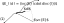
\includegraphics[width=0.25\textwidth]{img/2.png}
    %\caption{}
    %\label{fig:}
\end{figure}

\noindent
Из этих уравнений легко получить, что
\begin{equation}
    \left\{\begin{aligned}
        \frac{\partial U}{\partial z} &= - \frac{L_0}{c^2} \frac{d I}{d t} \\
        \frac{\partial I}{\partial z} &= - C_0 \frac{\partial U}{\partial t} 
    \end{aligned}\right.
    \hspace{0.5cm} \Rightarrow \hspace{0.5cm} 
    \boxed{
        \frac{\partial^2 U}{\partial t^2}  = \frac{c^2}{L_0 C_0} - \frac{\partial^2 V}{\partial z^2} 
    }.
\end{equation}
Решение аналогично будем искать в виде
\begin{equation}
    V = f_1 (z - vt) + f_2 (z + vt),
    \hspace{0.5cm} \Rightarrow \hspace{0.5cm} 
    v = \frac{c}{\sqrt{L_0 C_0}}.
\end{equation}
Кстати, если это всё посчитать для коаксиального кабеля, то
\begin{equation*}
    L_0 = 2 \mu \ln \frac{R_2}{R_1} , \hspace{0.5cm} 
    C_0 = \frac{\varepsilon}{2 \ln \frac{R_2}{R_1} },
    \hspace{0.5cm} \Rightarrow \hspace{0.5cm} 
    v = \frac{c}{\sqrt{\mu \varepsilon}}.
\end{equation*}


\subsubsection*{Коэффициент стоячей волны (standing wave ratio)}
Коэффициент стоячей волны -- отношение наибольшего значения амплитуды напряжённости электрического или магнитного поля стоячей волны в пучностях линии передачи к амплитуде в узлах.
КСВ является мерой согласования нагрузки (например, антенны) с линией передачи.

Наибольшее и наименьшее значения амплитуды соответсвенно равны
\begin{equation*}
    A_{\text{max}} = A_{\text{inc}} + A_{\text{ref}}, \hspace{0.5cm} 
    A_{\text{min}} = A_{\text{inc}} - A_{\text{ref}},
    \hspace{0.5cm} \Rightarrow \hspace{0.5cm} 
    \text{КСВ} = \frac{A_{\text{inc}} + A_{\text{ref}}}{A_{\text{inc}} - A_{\text{ref}}} = 
    \frac{1 + |\Gamma|}{1 - |\Gamma|},
\end{equation*}
где $|\Gamma|$ -- коэффициент отражения.

\subsubsection*{Согласованная нагрузка}
Рассмотрим длинную линию, пусть в цепи 
\begin{equation*}
    U = U_0 \cos \left(\omega_0 t - kz\right),  \hspace{0.5cm} 
    I = I_0 \cos \left(\omega_0 t - kz\right).
\end{equation*}
Сделаем следующий трюк. Возьмем, и продолжим линию до бесконечности, от которой, очевидно, ничего не отразится. Соотвественно нас интересует поиск эквивалентного импеданса системы. 
\begin{align*}
    U^* = U_0 \exp\left(i(\omega_0 t - kz)\right) &= U_0 e^{ikz} e^{-i\omega_0 t}, \\
    I^* = I_0 \exp\left(i(\omega_0 t - kz)\right) &= I_0 e^{ikz} e^{-i\omega_0 t}.
\end{align*}
Подставив эти выражения в волновое уравнение, и получим
\begin{equation*}
    ik U^* = i \omega_0 I^*,
    \hspace{0.5cm} 
    Z^* = U^* / I^* = \frac{\omega_0}{k},
    \hspace{0.5cm} \Rightarrow \hspace{0.5cm} 
    R = \frac{1}{c} \sqrt{\frac{L_0}{C_0}},
    \text{\ \ --- \ \ \textit{согласованная нагрузка}}.
\end{equation*}
То есть при наличии такого сопротивления на конце линии не будет никакого отражения. 




\sbsnum{25}{Формулы гладкой замены переменных в интеграле Лебега от функции}
\subsubsection*{Уравнение непрерывности}
\begin{to_def}[Предмет рассмотрения]
	Ввиду макроскопического рассмотрения \textit{жидкости}(газы) в гидродинамике представлется как сплошная среда, то есть малый элемент объёма жидкости содержит ещё достаточно больше количество молекул, относительно межмолекулярного расстояния.
\end{to_def}

Для описания движения жидкости требуется задать распределение скорости жидкости $\vc{v} = \vc{v}(x,y,z,t)$ и какие-либо её две термодинамические величины, как, например, плотность и давление. Важно отметить, что все эти величины относятся не к отдельной частице, а к точке в пространстве в определенное время.

\begin{to_thr}[Уравнение непрерывности]
\phantom{239}

\begin{proof}[$\triangle$]
	В маленьком объёме $V_{0}$ количество жидкости есть $\int_{V_0} \rho d V$.
	Через элемент поверхности, ограничивающей $V_0$, в единицу времени протекает $\rho \vc{v} \cdot d \vc{f}$ жидкости --- положительно или отрицательное число, в зависимости от того, вытекает или втекает жидкость соответственно.
	Тогда приравниваем для вытекания жидкости два наших рассуждения:
	\begin{equation*}
		- \frac{\partial}{\partial t} \int \rho d V =  \oint \rho \vc{v} \cdot d \vc{f}
		\hspace*{0.5 cm} 
		\Rightarrow 
		\hspace*{0.5 cm}
		\int \left(\frac{\partial \rho}{\partial t} + \div \rho \vc{v}\right)d V = 0
		\hspace*{0.5 cm}
		\Rightarrow
		\hspace*{0.5 cm}
		\frac{\partial \rho}{\partial t} + \div \rho \vc{v} = 0.
	\end{equation*}
	Последнее следует из того, что равенство должно иметь для любого объёма, таким образом получили искомое \textit{уравнение непрерывности}.
\end{proof}
	
\end{to_thr}

\subsubsection*{Уравнение Эйлера}

\begin{to_thr}[Уравнение Эйлера]
\phantom{239}

\begin{proof}[$\triangle$]
	Выделим в жидкости некоторый объём, полная сила, действующая на этот объём: $- \oint p d \vc{f} = - \int \grad p d V$, где интеграл из взятого по поверхности объёма преобразуется в сам рассматриваемый объём.
	Таким образом получили, что на единицу объёма жидкости будет действовать сила:
	\begin{equation*}
		\rho \frac{d \vc{v}}{d t} = - \grad p.
	\end{equation*}
	Однако стоящая здесь скорость определяет изменение скорости именно элемента объёма, а не точки в пространстве.
	Запишем это изменение скорости:
	\begin{equation*}
		d \vc{v} 
		=
		 \frac{\partial \vc{v}}{\partial t} d t + \frac{\partial \vc{v}}{\partial x^i} d x^i 
		= 
		\frac{\partial \vc{v}}{\partial t} d t + (d \vc{r} \cdot \nabla) \vc{v}
		\hspace*{1 cm}
		\Rightarrow
		\hspace*{1 cm}
		\frac{\partial \vc{v}}{\partial t} + (\vc{v} \nabla) \vc{v} = - \frac{1}{\rho} \grad p.
	\end{equation*}
	Последнее и есть искомое уравнение Эйлера.
\end{proof}
\end{to_thr}

Если же жидкость движется во внешнем поле тяжести, то, на каждый элемент объёма будет действовать сила, которая просто добавится к изначальному уравнению: 
\begin{equation*}
	\frac{\partial \vc{v}}{\partial t} + (\vc{v} \nabla) \vc{v} = - \frac{\nabla p}{\rho} + \vc{g}.
\end{equation*}

\subsubsection*{Уравнение Навье-Стокса}

Чтобы нормально учесть вязкость, нужно поговорить про \textit{поток импульса}.
Импульс единицы объёма жидкости есть $\rho \vc{v}$, скорость изменения его компоненты:
\begin{equation*}
	\frac{\partial}{\partial t} \rho v^i = \rho \frac{\partial v^i}{\partial t} + \frac{\partial \rho}{\partial t} v^i.
\end{equation*}
Уравнения непрерывности и Эйлера запишутся в тензорном виде:
\begin{equation*}
	\frac{\partial \rho}{\partial t} = - \frac{\partial (\rho v^k)}{\partial x^k},
	\hspace*{0.5 cm}
	\hspace*{0.5 cm}
	\frac{\partial v^i}{\partial t} = - v^k \frac{\partial v^i}{\partial x^k} - \frac{1}{\rho} \delta^{i k} \frac{\partial p}{\partial x^k}.
\end{equation*}
Тогда получим:
\begin{equation*}
	\frac{\partial}{\partial t} \rho v^i 
	= 
	- \rho v^k \frac{\partial v^i}{\partial x^k} -  \delta^{i k} \frac{\partial p}{\partial x^k} - v^i \frac{\partial \rho v^k}{\partial x^k} 
	=
	-\delta^{i k} \frac{\partial p}{\partial x^k} - \frac{\partial}{\partial x^k} \rho v^i v^k
	= - \frac{\partial \Pi^{i k}}{\partial x^k}.
\end{equation*}
\begin{to_def}
	$\Pi^{i k} $ --- \textit{тензор плотности потока импульса}:
	$
		\Pi^{i k} = p \delta^{i k} + \rho v^i v^k.
	$
\end{to_def}

Таким образом уравнение Эйлера у нас записалось в виде:
$
	\frac{\partial}{\partial t} \rho v^i = - \frac{\partial \Pi^{i k}}{\partial x^k}.
$
Поток импульса представляет собой чисто обратимый перенос импульса, связанный с просто механическим передвижением различных участков жидкости и с действующими в жидкости силами давления.
\textit{Вязкость} (внутреннее трение) жидкости проявляется в наличии ещё дополнительного, необратимого переноса импульса из мест с большой скоростью в места с меньшей.

Поэтому уравнение движения вязкой жидкости можно получить, прибавив к идеальному потоку импульса дополнительный член $\sigma^{i k}_{visc}$, определяющий такой вязкий перенос:
$
\Pi^{i k} = p \delta^{i k} + \rho v^i v^k - \sigma^{i k}_{visc} = - \sigma^{i k} + \rho v^i v^k.
$
\begin{to_def}
	Таким образом: $\sigma^{i k} = - p \delta^{i k} + \sigma^{i k}_{visc}$ называют \textit{тензором напряжений}, а $\sigma^{i k}_{visc}$ --- вязким тензором напряжений.
\end{to_def}

Чтобы написать выражение для вязкого напряжения сделаем пару оговорок. 
\textit{Во первых}, градиенты скорости движения участков жидкости относительно друг друга не велики, тогда $\sigma^{i k}_{visc}$ зависит лишь от первых производных скорости по координатам, линейно. \textit{Во вторых}, не зависящие от первых производных величины должны обращаться в нуль как для скорости потока $\vc{v} = \const$ и тензор должен быть нулевым. \textit{В третьих}, $\sigma^{i k}_{visc} = 0$ когда жидкость совершает целое равномерное вращение, поскольку никакого внутреннего трения тогда не будет.
Для такого равномерного вращения с $\vc{v} = [\vc{\omega} \vc{r}]$ линейными комбинациями производных обращающимися в нуль будут: $\frac{\partial v^i}{\partial x^k} + \frac{\partial v^k}{\partial x^i}$.

Это всё даёт нам мотивацию для не шибко сильных потоков несжимаемой жидкости согласится с Сэром Исааком Ньютоном, и написать тензор вязкого напряжения, как \textit{тензор скорости деформации}:
\begin{equation*}
	\sigma^{i k}_{visc} = \eta \left(\frac{\partial v^i}{\partial x^k} + \frac{\partial v^k}{\partial x^i}\right),
	\hspace*{1 cm}
	\Rightarrow
	\hspace*{1 cm}
	\sigma^{i k} = - p \delta^{i k} + \eta \left(\frac{\partial v^i}{\partial x^k} + \frac{\partial v^k}{\partial x^i}\right).
\end{equation*}
А уравнение Эйлера тогда для несжимаемой жидкости запишется:
\begin{equation*}
	\rho \left(\frac{\partial v^i}{\partial t} + v^k \frac{\partial v^i}{\partial x^k}\right)
	=
	- \delta^{i k} \frac{\partial p}{\partial x^k} + \frac{\partial}{\partial x^k} \left[\eta \left(\frac{\partial v^i}{\partial x^k} + \frac{\partial v^k}{\partial x^i}\right)\right].
\end{equation*}
а в более человеческом, привычном глазу, виде \textit{уравнение Навье-Стокса для несжимаемой жидкости}:
\begin{equation*}
	\frac{\partial \vc{v}}{\partial t} + (\vc{v} \triangle) \vc{v} = - \frac{1}{\rho} \grad p + \frac{\eta}{\rho} \Delta \vc{v}.
\end{equation*}
\begin{to_def}
	Коэффициент $\eta$ называется --- \textit{динамическим коэффициентом вязкости}, а отношение $\eta/\rho = \nu$ --- \textit{кинематической вязкостью}.
\end{to_def}


\newpage 


%%%%%%%%%%%%%%%%%%%%%%%%%%%%%%%%%%%%%%%%%%%%%%%%%%%%%%%%%%%%%%%%%%%%%%%%%%%%%%%%%%%
\section*{Многообразия (с краем) и формула Стокса}
\setcounter{section}{7}
\addcontentsline{toc}{section}{Многообразия (с краем) и формула Стокса}
%%%%%%%%%%%%%%%%%%%%%%%%%%%%%%%%%%%%%%%%%%%%%%%%%%%%%%%%%%%%%%%%%%%%%%%%%%%%%%%%%%%

\sbsnum{26}{Вложенные многообразия}
Напишем систему уравнений, соответствующую уравнениям Лагранжа первого рода:

\begin{equation}
    \sum_{\nu=1}^N \vc{a}_{\beta \nu} (\vc{r}_1, \ldots, \vc{r}_N, t) \cdot \vc{v}_\nu + a_\beta  (\vc{r}_1, \ldots, \vc{r}_N, t) = 0,
    \hspace{0.5cm} (\beta = 1, \ldots, s)
\end{equation}
$$
    f_\alpha (\vc{r}, t) = 0, \hspace{0.5cm} (\alpha = 1, \ldots, r),
$$
\begin{align}
    \sum_{\nu=1}^N \frac{\partial f_\alpha}{\partial \vc{r}_\nu} \cdot d \vc{r}_\nu + \frac{\partial f_\alpha}{\partial t} d t &= 0,
    \hspace{0.5cm} &(\alpha = 1, \ldots, r), \\
    \sum_{\nu=1}^N \vc{a}_{\beta\nu} \cdot d \vc{r}_\nu + a_\beta d t &= 0,
    \hspace{0.5cm} &(\beta = 1, \ldots, s).
\end{align}



Взяв выражения для виртуальных перемещений всегда можно получить силы реакции так называемым методом \textit{множителей Лагранжа}:
\begin{equation*}
    \sum_{\nu=1}^N \left(\vc{R}_\nu - \sum_{i = 1}^r \lambda_i \frac{\partial f_i}{\partial \vc{r}_\nu} - \sum_{j = 1}^s \mu_j \alpha_{j \nu}\right) \delta \vc{r}_\nu = 0
    \hspace*{1 cm}
    \Rightarrow
    \hspace*{1 cm}
    \vc{R}_\nu = \sum_{i = 1}^r \lambda_i \frac{\partial f_i}{\partial \vc{r}_\nu} + \sum_{j = 1}^s \mu_j \alpha_{j \nu}.
\end{equation*}
Полученные выражения для реакций идеальных сил через неопределенные множители Лагранжа $\lambda_i $ и $\mu_j $ можно подставить в исходное уравнение связей, получим \textit{уравнения Лагранжа первого рода}:
\begin{equation*}
    m_\nu \vc{w}_\nu = \vc{F}_\nu + \sum_{i = 1}^r \lambda_i \frac{\partial f_i}{\partial \vc{r}_\nu} + \sum_{j = 1}^s \mu_j \alpha_{j \nu}.
\end{equation*}

\sbsnum{27}{Абстрактное определение гладкого многообразия}
\subsubsection*{Преломление и поглощение волн}

Пусть есть некоторое внешнее поле $E = E_0 e^{i(\omega t - kz)}$. Посмотрим на электрон на орбите атома,
\begin{equation*}
    m \ddot{z} = - k z - \beta \dot{z} + E_0 \cdot e^{-i(\omega t - kz)},
    \hspace{0.5cm} \overset{p = e z}{\Rightarrow}  \hspace{0.5cm} 
    \ddot{p} + 2 \delta \dot{p} + \omega_0^2 p = \frac{eE_0}{m} e^{-i(\omega t - kz)},
\end{equation*}
будем искать решения вида $p = p_0 e^{i\omega t}$, тогда
\begin{equation*}
    p = \frac{eE_0}{m} \frac{
    1
    }{
    (\omega_0^2 - \omega_2) - 2 \delta \omega i 
    } 
    e^{-i(\omega t - kz)}.
\end{equation*}
Вспомним, что $D$ равно
\begin{equation*}
     D = E + 4 \pi N p = 
     \bigg(
     \underbrace{
     1 + \frac{4\pi N e^2}{m} \cdot 
     \frac{1}{(\omega_0^2 - \omega^2) - 2 \delta \omega i} 
     }_{\varepsilon}
    \bigg) E.
\end{equation*}
По определению $n = \sqrt{\varepsilon}$, то есть
\begin{equation*}
    n^2 = \varepsilon = 1 + \frac{4\pi N e^2}{m} \cdot 
     \frac{1}{(\omega_0^2 - \omega^2) - 2 \delta \omega i}.
\end{equation*}

В случае проводника $\omega_0 = 0$, к тому же $2 \delta = 1 / \tau$, где $\tau$ -- характерное время затухания. Запишем, что
\begin{equation*}
    j = \sigma E, \hspace{0.5cm} j = N e v,
    \hspace{0.5cm} 
    v = \frac{eM}{m} \tau
    \hspace{0.5cm} \Rightarrow \hspace{0.5cm} 
    \tau = \frac{m\sigma}{Ne^2}. 
\end{equation*}
Тогда для проводника
\begin{equation*}
    n^2 = 1 - \frac{4\pi\sigma}{\omega i (1 -i \omega \tau)}.
\end{equation*}
Рассмотрим два случая, когда $\omega \tau \ll 1$, и $\omega \tau \gg 1$. 

\subsubsection*{Скин-эффект}


Первый случай приводит нас к явлению скин-эффекта.
\begin{equation*}
    n^2 = 1 - \frac{4\pi\sigma}{\omega i (1 -i \omega \tau)} 
    \approx
    1 - \frac{4\pi \sigma}{\omega i} \approx i \frac{4 \pi \sigma}{\omega},
    \hspace{0.5cm} \Rightarrow \hspace{0.5cm} 
    n = \left(\frac{1 + i}{\sqrt{2}}\right) \sqrt{\frac{4\pi\sigma}{\omega}}
    = \sqrt{\frac{2\pi\sigma}{\omega} } (1 + i)
    .
\end{equation*}
Посмотрим к чему это приводит. 
\begin{equation*}
    E = E_0 e^{-i(\omega t - kz)}, \hspace{0.5cm} 
    k = \frac{\omega}{c} \sqrt{\varepsilon \mu} = \frac{\omega}{c} n.
\end{equation*}
Тогда
\begin{equation*}
    E = E_0 e^{-i(\omega t - \frac{n}{c} z)} = E_0
    e^{-i \omega t} \exp\left(
        i \frac{\omega}{c} \sqrt{\frac{2\pi\sigma}{\omega} }z
    \right)
    \exp\left(
        - \frac{\omega}{c} \sqrt{\frac{2\pi\sigma}{\omega} }
    \right).
\end{equation*}
Появился множитель, соответсвующий экспоненциальному затуханию
\begin{equation*}
    z_0 = \sqrt{\frac{c^2}{2\pi \sigma \omega} },
\end{equation*}
где на $z_0$ происходит затухание в $e$ раз. 


\subsubsection*{Прозрачность металлов}

Первый случай приводит к прозрачности металлов.
\begin{equation*}
    n^2 = 1 - \frac{4\pi\sigma}{\omega i (1 -i \omega \tau)} 
    \approx
    1 - \frac{4\pi\sigma}{\omega^2 \tau} = 1 - \frac{\omega_{\text{p}}^2}{\omega^2} 
    ,
    \omega_{\text{p}}:2 = 
    \frac{4 \pi \sigma}{\tau} = \frac{4 \pi N e^2}{m}.
\end{equation*}
То есть при $\omega < \omega_{\text{p}}$ происходит отражение, а при $\omega > \omega_{\text{p}}$ металл становится прозрачным, то есть похожим на диэлектрик. 






% \subsubsection*{Бонус о плазме}







\sbsnum{28}{Диф-формы, векторные поля и \texorpdfstring{$d$}{d} на многообразии}

Легко получить соотношение вида
\begin{equation}
    \sum_{i=1}^N \left(
        \vc{F}_i - m_i \vc{\mathrm{w}}_i
    \right) \cdot \delta \vc{r}_i = 0.
\end{equation}
Данное соотношение является необходимым и достаточным условием для того, чтобы движение, совместимое с идеальными связями, отвечало данной системе активных сил $\vc{F}_i$. Оно получило название \textbf{общего уравнения динамики} или \textit{дифференциальным вариационным принципом Даламбера-Лагранжа}.

\begin{to_thr} [принцип Даламбера-Лагранжа]
Верно, что
\begin{equation*}
    m_i \vc{\mathrm{w}}_i = \vc{F}_i + \vc{R}_i,
    \hspace{0.5cm} \Rightarrow \hspace{0.5cm} 
    \sum_i \left(
       \vc{F}_i -  m_i \vc{\mathrm{w}}_i
    \right) \cdot \delta \vc{r}_i = 0.
\end{equation*}
\end{to_thr}

Аналогично можно сформулировать \textit{принцип Журдена}
\begin{equation}
    \sum_{i=1}^N \left(
        \vc{F}_i - m_q \vc{\mathrm{w}}_i
    \right) \cdot \delta  \vc{v}_i = 0,
\end{equation}
и \textit{принцип Гаусса}:
\begin{equation}
    \sum_{i=1}^N \left(
        \vc{F}_i - m_q \vc{\mathrm{w}}_i
    \right) \cdot \delta \vc{\mathrm{w}}_i = 0,
\end{equation}
где $\delta \vc{\mathrm{w}}_i = \vc{\mathrm{w}}^*_{i_1} - \vc{\mathrm{w}}^*_{i_2}$ не обязательно малая величина. 

Замечая, что $m_i = \const$, а $\vc{F}_i = \vc{F}_i (p, q)$, то последнее уравнение перепишется в виде
\begin{equation*}
    Z = \frac{1}{2} \sum_{i=1}^N m_i 
    \left(
        \vc{\mathrm{w}}_i - \frac{\vc{F}_i}{m_i} 
    \right)^2,
    \hspace{1cm} 
    \delta Z = 0,
\end{equation*}
где величина $Z$ называется принуждением или мерой принуждения. К слову она не просто стационарна для истинных движений. 

\texttt{Истинным является движение с минимальной мерой принуждения.} Другими словами \textit{несвободная система совершает движение, наиболее близкое к свободному}. 

\begin{to_def} 
    Будем считать, что $q^0 \in M$ -- \textit{точка равновесия}, если при $\dot{q}^0 \equiv \dot{q}(0) \equiv 0$ приводит к $q(t) = q^0$. 
\end{to_def}

В таком случае верен следующий принцип:

\begin{to_thr}[принцип Лагранжа]
    Для того, чтобы точка была положением равновесия на $t \in [t_1, t_2]$ необходимо и достаточно, чтобы сумма элементарных работ на $\forall$ виртуальных перемещениях всех активных сил была равна нулю.
    \begin{equation}
        \delta A \big|_0 = 0 
        \hspace{0.5cm} 
        \delta A = \sum_i \vc{F}_i \cdot \delta \vc{r}_i,
        \hspace{0.5cm} (t\in[t_1, t_2])
    \end{equation}
    что является \textbf{общим уравнением статики}.
\end{to_thr}

Этот принцип можно рассматривать, как дракона с тремя головами. Вот если система \textbf{голономная}, то
\begin{equation*}
    \delta A = Q_i \delta q_i 
    \hspace{0.5cm} \Rightarrow \hspace{0.5cm} 
    Q_i = 0 \ \forall i.
\end{equation*}
Если система \textbf{консервативная}, то
\begin{equation*}
    Q_1 = - \frac{\partial P}{\partial q^i} 
    \hspace{0.5cm} \Rightarrow \hspace{0.5cm} 
    \text{положение равновесия --- стационарная точка потенциала}.
\end{equation*}
Если же у нас \textbf{твёрдое тело}, тогда
\begin{equation*}
    \delta A = \left(
        \vc{R}^{\text{внеш}} \cdot \vc{v}_O
    \right) \d t + 
    \left(
        \vc{M}_O^{\text{внеш}} \cdot \vc{\omega}
    \right) dt
    \hspace{0.5cm} \Rightarrow \hspace{0.5cm} 
    \left\{\begin{aligned}
        \vc{R}^{\text{внеш}} &= 0 \\
        \vc{M}^{\text{внеш}} &= 0 \\
    \end{aligned}\right.
\end{equation*}



\sbsnum{29}{Гладкие отображения многообразий}

\begin{to_def} 
    Функция $f \colon M \mapsto \mathbb{R}$ называется \textit{гладкой функцией на многообразии}, $f \in C^{\infty}(M)$, если в каждой координатной карте $\varphi \colon U \mapsto \mathbb{R}^n$ эта функция ($f \circ \varphi^{-1}$) является гладкой функцией на образе $\varphi(U)$.
\end{to_def}



\begin{to_def} 
    \textit{Гладкой структурой} на топологическом пространстве называется максимальный по включению атлас, с которым пространство становится многообразием. 
\end{to_def}


\begin{to_def} 
    \textit{Гладким отображением} между многообразиями $f \colon M \mapsto N$ размерностей $m$ и $n$ называется непрерывное отображение, которое в окрестности каждой точки, в достаточно малых координатных картах, выглядит как гладкое отображение из $\mathbb{R}^m$ в $\mathbb{R}^n$.
\end{to_def}


\begin{to_def} 
    Гладкое обратимое отображение $f \colon M \mapsto N$ с обратным гладким назовётся \textit{диффеоморфизмом многообразий}. 
\end{to_def}

\begin{to_tas} 
\label{task_6.131} % + текст с 227 страницы.
    Если взять некоторое \textit{компактное} гладкое многообразие $M$ (область параметров) и гладкое отображение $f \colon M \mapsto \mathbb{R}^n$, такое, что $\rg Df_p = \dim M$ $\forall p$, то $f(M)$ будет вложенным многообразием.     
\end{to_tas}

\begin{to_lem} 
    Для гладкого отображения $f \colon M \mapsto \mathbb{R}^n$ с $\rg Df \equiv m = \dim M$, для всякой $p \in M$ найдётся окрестность $U \ni p$ такая, что $f(U)$ в некоторой криволинейной системе координат в окрестности $f(p)$ является открытым подмножеством стандартно вложенного $\mathbb{R}^m \subseteq \mathbb{R}^n$. 
\end{to_lem}


\sbsnum{30}{Ориентируемость многообразия}
\begin{to_def} 
    Гладкое многообразие $M$ называется \textit{ориентируемым}, если можно выбрать покрывающий атлас так, что якобианы замен координат между любыми двумя картами атласа будут положительными. 
\end{to_def}

Если в исходном атласе был задан некоторый объект, например векторное поле $X$, то во всякой новой карте $\psi$ мы тоже будем иметь векторное поле, собранное из прямых образов $(\psi  \circ \varphi^{-1})_* X_\varphi$ полученных с имеющихся карт $\varphi$ и образов $X_\varphi$ в них.

\begin{to_def} 
    \textit{Ориентацией гладкого многообразия} $M$ называется атлас с положительными якобианами перехода между картами, максимальный по включению среди всех таких атласов. 
\end{to_def}

\begin{to_lem} 
    Связное многообразие либо неориентируемо, либо допускает два класса ориентации. 
\end{to_lem}

\begin{to_lem} 
    Многообразие $M$ размерности $n$ ориентируемо тогда и только тогда, когда существует дифференциальная форма $\nu \in \Omega^n (M)$, которая ни в одной точку не равна нулю.
\end{to_lem}

\begin{to_lem} 
\label{zorich_cXV.p2.lem4} % см. страницу 308
    Многообразие ориентируемо тогда и только тогда, когда на нём не существует противоречивой (дезориентирующей) цепочки карт.
\end{to_lem}

\begin{to_def} 
    Для $n$-мерного ориентированного многообразия с краем $M$ введём ориентацию на его крае $\partial M$ следующим образом. Пусть карта $M$ с координатами $x_1, \ldots, x_n$ соответсвует ориентации $M$, причём образ отображения карты удовлетворяет неравенству $x_1 \leq 0$, а образ края соответствует равенству $x_1 = 0$. Тогда карта на соответствующей части $\partial M$ из координат $x_2, \ldots, x_n$ по определению объявляется положительной. Если же многообразие в этой карте задано неравенством в другую сторону, $x_1 \geq 0$, то карта $x_2, \ldots, x_n$ на его краю по определению объявляется отрицательной. 
\end{to_def}

\begin{to_lem} 
    Предыдущее определение корректно задаёт ориентацию на $\partial M$. 
\end{to_lem}








\sbsnum{31}{Определение интеграла диф-формы по ориентированному многообразию}
\begin{to_lem}[Разбиение единицы в окрестности компакта на многообразии]
     Пусть $M$ -- гладкое многообразие, а $K \subseteq M$ -- его компактное подмножество. Для любого покрытия $\{U_\alpha\}_\alpha$ компакта $K$ открытыми множествами найдётся набор неотрицательных гладких функций $\{\rho_\alpha\}_\alpha$ с компактными носителями $\mathrm{supp}\, \rho_\alpha$ таких, что
\begin{equation*}
    \forall \alpha \ \textnormal{supp}\, \rho_\alpha \subset U_\alpha,
\end{equation*}
    только конечное число из них отлично от нуля и
    $\sum_\alpha \rho_\alpha (x) \equiv 1$
    в некоторой окрестности $K$.
\end{to_lem}

\begin{to_def} 
    Интеграл дифференциальной формы $\nu \in \Omega_{\text{c}}^n (M)$ с компактным носителем по ориентированному $n$-мерному многообразию $M$ определяется с помощью разбиения единицы в окрестности носителя $\nu$ 
    \begin{equation*}
         \rho_1 + \ldots + \rho_m = 1,
     \end{equation*} 
     подчиненного некоторому набору положительно ориентрированных карт как
     \begin{equation*}
         \int_M \nu = \sum_i \int_M \rho_i \nu_i,
     \end{equation*}
     где интегралы справа рассматриваются в координатных картах, содержащих носители соответствующих $\rho_i$.
\end{to_def}

\begin{to_lem} 
    Определение интеграла не зависит от выбора системы положительных карт в данной ориентации и подчиненного им разбиения единциы. 
\end{to_lem}





\sbsnum{32}{Общая формула Стокса} 
Подставим разложение кинетической энергии в уравнения Лагранжа, оставив только слагаемые с обобщёнными ускорениями $f_j (q, \dot{q}, t) = a_{jk} \ddot{q}^j$. 
\begin{equation*}
    T = \frac{1}{2} \sum_\nu m_\nu \dot{\vc{r}}_\nu^2 = \frac{1}{2} \sum_\nu
    \left(
        \frac{\partial \vc{r}_\nu}{\partial q^j} \dot{q}^j + \frac{\partial \vc{r}_\nu}{\partial t} 
    \right)^2 = 
    \frac{1}{2} 
    \bigg[
    \underbrace{
        a_{jk} \dot{q}^j \dot{q}^k
    }_{
        2T_2
    } +
    \underbrace{
        a_j \dot{q}^j
    }_{
        2T_1
    } +
    \underbrace{
        a_0
    }_{
        2T_0
    }
    \bigg],
\end{equation*}
где коэффициенты, соответственно, равны 
\begin{equation*}
    a_{jk}(q, t) = \sum_\nu m_\nu \frac{\partial \vc{r}_\nu}{\partial q^j} \cdot \frac{\partial \vc{r}_\nu}{\partial q^k},
    \hspace{0.5cm} 
    a_j(q, t) = \sum_\nu m_\nu \frac{\partial \vc{r}_\nu}{\partial q^j} \cdot \frac{\partial \vc{r}_\nu}{\partial t},
    \hspace{0.5cm} 
    a_0 = \sum_\nu m_\nu 
    \left(
    \frac{\partial \vc{r}_\nu}{\partial t} 
            \right)^2.
\end{equation*}
Для склерономных систем $\partial \vc{r}_\nu / \partial t = 0$, соотвественно $T = a_{jk} \dot{q}^j \dot{q}^k$, при чём $a_{jk} \equiv a_{jk} (q)$.

Теперь подставим значение $T$ в уравнения Лагранжа, и получим, что
$
    a_{ik} \ddot{q}^k = f_i,
$
где $f_1 = f_1(q, \dot{q}, t)$. Уравнений в системе $n$, причём $a_{jk}$ является положительно определенной формой\footnote{
    \red{Требует отдельного доказательства.}
}, соответственно невырожденной. 

\begin{to_thr} 
    Уравнения Лагранжа второго рода разрешимы относительно обобщенных ускорений 
\end{to_thr}
 

\sbsnum{33}{Частные случаи формулы Стокса}
 % \renewcommand{\labelenumi}{\Roman{enumii}}
\begin{enumerate}[label={$\mathbb{R}^\text{\arabic*}$.}]
    \item Формула Стокса для ориентированной кривой с началом в точке $p$ и концом в точке $q$ сводится к 
    \begin{equation*}
        \int_\gamma \d f = f(q) - f(p).
    \end{equation*}
    \item Для компактного множества $G \subset \mathbb{R}^2$ с гладкой границей, ориентированного так, что при движении по $\partial G$ множество $G$ оказывается слева, верна \textit{формула Грина}
    \begin{equation*}
        \int_{\partial G} P \d x + Q \d y = \int_G
        \left(
            \frac{\partial Q}{\partial x} - \frac{\partial P}{\partial y} 
        \right) \d x \wedge d y.
    \end{equation*}
    \item Для компактного множества $G \subset \mathbb{R}^3$ с гладкой границей (край в $\mathbb{R}^3$) верна \textit{формула Гаусса-Остроградского}
    \begin{equation*}
        \int_{\partial G} P \d y \wedge d z 
        + Q \d z \wedge dx 
        + R \d x \wedge dy = 
        \int_G
        \left(
            \frac{\partial P}{\partial x} +
            \frac{\partial Q}{\partial y} +
            \frac{\partial R}{\partial z} 
        \right) \d x \wedge d y \wedge d z.
    \end{equation*}
\end{enumerate}


Кривую можно считать не бесконечно гладкой, а всего лишь кусочно непрерывно дифференцируемой, формула всё равно остаётся верной. С помощью предельного перехода также обобщается случай с $\simeq \mathbb{R}^2$ до множества с кусочно $C^2$ границей.

Вообще формула Стокса верна не только для вложенных двумерных многообразий, но и для всякого образа гладкого отображения $f \colon D \mapsto  \mathbb{R}^3$ области $D \subset \mathbb{R}^2$ с кусочно гладкой границей, если интегралы мы понимаем как интегралы обратных образов $f^*(\alpha)$ и $f^*(d\alpha)$ по $\partial D$ и $D$ соответственно. Для практических применений полезно ослабить условие гладкости $f$ до $C^2$ (в интеграле, в координатном представлении, используются производные $f$ не более чем первого порядка).


% Кривую 

 % дописать материал из Зорича

\sbsnum{34}{Потенциал диф-форм}
Физический потенциал силового поля в математический терминах означает поиск $f \in C^\infty (M) \colon \d f = \alpha$ для заданной силы $\alpha \in \Omega^1(M)$

\begin{to_thr}
	Необходимым и достаточным условием наличия потенциала у непрерывной $\alpha \in \Omega^1(M)$, для гладкого $M$, является независимость $\int_\gamma \alpha$ от выбора между двумя точками кусочно-гладкой кривой $\gamma$.

	Эквивалентно можно потребовать равенства нулю интегралов по всем замкнутым кусочно-гладким кривым.
	\label{thr_7.1}
\end{to_thr}

Удобным на практике необходимым условием существования потенциала у $\alpha \in \Omega^1(M)$ является $\d \alpha = 0$ (т.к. $\d (\d u) = 0$).
Однако этого не достаточно, так например в открытой $U = \mathbb{R}^2 \backslash \{ 0 \}$:
\begin{equation*}
	\alpha = \frac{x \d y - y \d x}{x^2 + y^2}
	\hspace*{0.5 cm} \leadsto \hspace*{0.5 cm}
	\d \alpha = 0,
	\hspace*{0.5 cm} \text{ но } \hspace*{0.5 cm}
	\oint_{S^1} \alpha = 2 \pi.
\end{equation*}

Далее в качестве упражнений оставлены следующие важные замечания:

\begin{to_tas}[Порядок точки относительно кривой]
Для замкнутой кусочно-гладкой $\gamma \in \mathbb{R}^2$, не проходящей через начало координат определим порядок начала координат относительно кривой:
\begin{equation*}
	w (\gamma, 0) - \frac{1}{2 \pi} \int_{\gamma} \frac{x \d y - y \d x}{x^2 + y^2},
\end{equation*}
и он не меняется при непрерывных деформациях кривой, при которых она не проходит через начало координат.
\end{to_tas}

\begin{to_tas}
	Порядок начала координат относительно кривой является целым.
\end{to_tas}

\begin{to_tas}
	Порядок начала координат относительно не проходящей через него нечётной кривой является нечётным числом. ($\gamma \colon \mathbb{S}^1 \rightarrow \mathbb{R}^2, \; \gamma(-u) = - \gamma(u)$).
\end{to_tas}

\begin{to_tas}
	Для замкнутой кривой на плоскости с всюду не нулевой скоростью $\int k(s) \d s = 2 \pi N, \; N \in \mathbb{Z}$.
\end{to_tas}

\begin{to_tas}[Лемма Жордана]
	Замкнутая кусочно-гладкая кривая $\gamma \subset \mathbb{R}^2$ без самопересечений делит плоскость на две связные части внутреннюю и внешнюю (можно усложнить и сформулировать для непрерывных кривых).
\end{to_tas} % дописать материал из Зорича

\newpage 


%%%%%%%%%%%%%%%%%%%%%%%%%%%%%%%%%%%%%%%%%%%%%%%%%%%%%%%%%%%%%%%%%%%%%%%%%%%%%%%%%%%
\section*{Элементы дифференциальной топологии}
\setcounter{section}{8}
\addcontentsline{toc}{section}{Элементы дифференциальной топологии}
%%%%%%%%%%%%%%%%%%%%%%%%%%%%%%%%%%%%%%%%%%%%%%%%%%%%%%%%%%%%%%%%%%%%%%%%%%%%%%%%%%%

\sbsnum{35}{Замкнутые и точные формы. Цепные гомотопии}
\subsubsection*{Преобразование Лежандра}

\begin{to_def} 
    В уравнениях Лагранжа второго рода движения голономной системы в потенциальном поле сил, функция Лагранжа зависит от $q, \ \dot{q}, \ t$ -- \textit{переменные Лагранжа}.
    Если в качестве параметров взять $q, \ p, \ t$, где $p_i$ -- \textit{обобщенные импульсы}\footnote{
        Обобщенный импульс $p_i$ -- ковектор, а  не вектор!
    }, определяемые как
    $
        p_i = {\partial L}/{\partial \dot{q}^i}.
    $
    То получим набор $q, \ p, \ t$ -- \textit{переменные Гамильтона}. 
\end{to_def}

В силу невырожденности $\partial L / (\partial \dot{q}^i \partial \dot{q}^j) = J_{p}$, то есть по \textit{теореме о неявной функции} эти равенства разрешимы относительно переменных $\dot{q}^i$. Через преобразование Лежандра естестественно ввести функцию
\begin{equation*}
    H(q, p, t) = p_i \dot{q}^i - L(q, \dot{q}, t),  \hspace{0.5cm} \dot{q} \equiv \dot{q}(q, p, t).
\end{equation*}

\subsubsection*{Уравнения Гамильтона}
% Маркеев, п.149.

Полный дифференциал функции Гамильтона можем выразиь двумя способами:
\begin{equation*}
    \left.\begin{aligned}
        d H &= \frac{\partial H}{\partial q^i} \d q^i + \frac{\partial H}{\partial p_i} \d p_i + \frac{\partial H}{\partial t} \d t,
        \\
        dH &= \dot{q}^i \d p_i - \frac{\partial L}{\partial q^i} \d q^i - \frac{\partial L}{\partial t} \d t.
    \end{aligned}\right\}
    \hspace{0.7cm} \Rightarrow \hspace{0.7cm} 
    \left.\begin{gathered}
        \frac{\partial H}{\partial t} = - \frac{\partial L}{\partial t} \\
        \frac{\partial H}{\partial p_i} = \dot{q}^i, \ \ 
        \frac{\partial H}{\partial q^i} = - \frac{\partial L}{\partial q^i}
    \end{gathered}\right.
    \hspace{0.7cm} \Rightarrow \hspace{0.7cm} 
    \left\{\begin{aligned}
        \frac{d q^i}{d t} &= \frac{\partial H}{\partial p_i}, \\
        \frac{d p_i}{d t} &= - \frac{\partial H}{\partial q^i}.    
    \end{aligned}\right.
\end{equation*}
Эти уравнения называются \textit{уравнениями Гамильтона}, или \textit{каноническими уравнениями}.


\subsubsection*{Физический смысл функции Гамильтона}

Пусть система натуральна, тогда $L = L_2 + L_1 + L_0$, и, соответсвенно,
\begin{equation*}
    H = \frac{\partial L}{\partial \dot{q}^i} \dot{q}^i - L.
\end{equation*}
По теореме Эйлера об однородных функциях
\begin{equation*}
    \frac{\partial L_2}{\partial \dot{q}^i} \dot{q}^i = 2 L_2,
    \hspace{1cm} 
    \frac{\partial L_1}{\partial \dot{q}^i} \dot{q}^i = L_1,
    \hspace{0.5cm} \Rightarrow \hspace{0.5cm} 
    H = L_2 - L_0.
\end{equation*}
пусть $T = T_2 + T_1 + T_0$, если силы имеют обычный потенциал $\Pi$, то $L_0 = T_0 - \Pi$, 
\begin{equation*}
    H = T_2 - T_0 + \Pi.
\end{equation*}
Если же силы имеют обобщенный потенциал $V = V_1 + V_0$, то $L_0 = T_0 - V_0$, и
\begin{equation*}
    H = T_2 - T_0 + V_0.
\end{equation*}
В случае натуральных и склерономных систем $T_1 = T_0 = 0$ и $T = T_2$, тогда $H = T + \Pi$. Т.е. для натуральных склерономных систем с обычным потенциалом сил функция Гамильтона $H$ представляет собой полную механическую энергию.

\subsubsection*{Интеграл Якоби}

Найдём полную производную $H$ по времени,
\begin{equation*}
    \frac{d H}{d t} = \frac{\partial H}{\partial q^i} \dot{q}^i + \frac{\partial H}{\partial p_i} \dot{p}_i + \frac{\partial h}{\partial t} = 
    \frac{\partial H}{\partial q^i} \frac{\partial H}{\partial p_i} - \frac{\partial H}{\partial p_i} \frac{\partial H}{\partial q^i} + \frac{\partial H}{\partial t} = \frac{\partial H}{\partial t},
    \hspace{0.5cm} \Rightarrow \hspace{0.5cm} 
    \frac{d H}{d t} = \frac{\partial h}{\partial t}.
\end{equation*}
Система называется \textit{обобщенно консервативной}, если $\partial H / \partial t = 0$, т.е $H(q^i, p_i) = h$, собственно, $H$ называют \textit{обобщенной полной энергией}, а поледнее равенство -- \textit{обобщенным интегралом энергии}.


\begin{to_def} 
    Для натуральной системы с обычным потенциалом сил, если $\partial H/ \partial t =0$, то
    \begin{equation*}
         H = T_2 - T_0 + \Pi = h = \const.
     \end{equation*} 
     Соотноешние, где $h$ -- произвольная постоянная, называют \textit{интегралом Якоби}.
\end{to_def}

Есть и другая формулировка для интеграла Якоби голономной склерономной системы. Действительно, при $\partial L / \partial t = 0$, интеграл Якоби перейдёт в
\begin{equation*}
    \frac{\partial H}{\partial t} = 0,
    \hspace{0.25cm} \Rightarrow \hspace{0.25cm} 
    \frac{d }{d t} \left(
        \frac{\partial L}{\partial \dot{q}^i} \dot{q}^i
    \right) = 0,
    \hspace{0.25cm} \Rightarrow \hspace{0.25cm} 
    \frac{\partial L}{\partial \dot{q}^i} \dot{q}^i = \const.
\end{equation*}



\subsubsection*{Уравнения Уиттекера}


Если $\partial H / \partial t = 0$, то $H(q, p) = h$, где $h = \const$ определяемая из н.у. В $2n$-мерном пространстве $q, \ p$ интеграл Якобми задаёт гиперповерхность, рассмотрим движение с $H = h$.

Такое движение описывается системой с $2n-2$ уравнений, причём она может быть записана в виде канонических уравнений. Пусть $\partial H / \partial p_1 \neq 0$, тогда
\begin{equation*}
    p_1 = - K(q^1, \ldots, q^n, p_2, \ldots, p_n, h),
    \hspace{0.5cm} \Rightarrow \hspace{0.5cm} 
    \left\{\begin{aligned}
        \dot{q}^i = \frac{\partial H}{\partial p_i}, \\
        \dot{p}_j = - \frac{\partial H}{\partial q^j}        
    \end{aligned}\right.
    \hspace{0.5cm} \Rightarrow \hspace{0.5cm} 
    \frac{d q^j}{d q^1} = \frac{
    \left(\dfrac{\partial H}{\partial p_j} \right)
    }{
    \left(\dfrac{\partial H}{\partial p_1} \right)
    },
    \hspace{0.5cm} 
    \frac{d p_j}{d q^1} = - \frac{
    \left(\dfrac{\partial H}{\partial q^j}\right)
    }{
    \left(\dfrac{\partial H}{\partial p_1} \right)
    },
\end{equation*}
для $j = 2,\ 3,\ \ldots,\ n$. Подставляя $p_1$ получим
\begin{align*}
    &\frac{\partial H}{\partial q^j} - \frac{\partial H}{\partial p_1} \frac{\partial K}{\partial q^j} = 0,
    &(j = 2, \ 3, \ \ldots, n);
    \\
    &\frac{\partial H}{\partial p_j} - \frac{\partial H}{\partial p_1} \frac{\partial K}{\partial p_j}  = 0,
    &(j = 2, \ 3, \ \ldots, n).
\end{align*}
Допиливая до надлежащего вида, окончательно находим
\begin{equation*}
    \frac{d q^j}{d q^1} = \frac{\partial K}{\partial p_j},
    \hspace{1cm} 
    \frac{d p_j}{d q_1} = - \frac{\partial K}{\partial q^j},
    \hspace{1cm} 
    (j = 2, \ 3, \ \ldots, n).
\end{equation*}
Эти уравнения описывают движения системы при $H = h = \const$, и называются \textit{уравнениями Уиттекера}. 

\subsubsection*{Уравнения Якоби}


Уравнения Уиттекера имеют структуру уравнений Гамильтона, соответственно их можно зписать в виде уравнений типа Лагранжа, при гессиане $K$ по $p$ неравным 0. Пусть $P$ -- преобразование Лежандра функции $K$ по $p_j$ ($j = 2, \ 3,\ \ldots,\ n$). Тогда
\begin{equation*}
    P = P(q^2, \ldots, q^n, \tilde q^2, \ldots, \tilde q^n, q^1, h) = \sum_{j = 2}^{n} \tilde q^j p_j - K,
\end{equation*}
где $\tilde q^{j} = d q^j / d q^1$. Величины $p_j$ выражаются через $\tilde q^2, \ \ldots, \ \tilde q_n$ из уравнений 
\begin{equation*}
    \tilde q^j = \frac{\partial K}{\partial p_j}, \hspace{0.5cm} 
    (j = 2, \ 3, \ \ldots, n),
\end{equation*}
т.е. из первых $n-1$ уравнений Уиттекера. При помощи функции $P$ эти уравнения могут быть записаны в эквивалентной форме:
\begin{equation*}
    \frac{d }{d q^1} \frac{\partial P}{\partial q_j'} - \frac{\partial P}{\partial q^j} = 0
    \hspace{1cm} (j = 2,\ 3,\ \ldots,\ n).
\end{equation*}
Это уравнения типа Лагранжа, называются \textit{уравнениями Якоби}.

Преобразовывая выражение для $P$ найдём, что
\begin{equation*}
    P = \sum_{j=2}^{n} q_j \tilde q^j + p_1 = 
    \sum_{i=1}^{n} p_1 \tilde q_i = \frac{1}{\dot{q}^1} \sum_{i=1}^{n} p_i \dot{q}^i = \frac{1}{\dot{q}^1} (L+H).
\end{equation*}
Тогда в случае консервативной системы $L = T - \Pi$, $H = T + \Pi$, и\footnote{
    \red{Пара выражений в выводе опущены.}
}
\begin{equation*}
    P = \frac{2T}{\dot{q}^1},
    \hspace{0.5cm} \Rightarrow \hspace{0.5cm} 
    P = 2 \sqrt{(h-\Pi) G}.
\end{equation*}



\sbsnum{36}{Когомологии де Рама}
В силу теоремы Пуанкаре (\ref{thr_poin}) любая замкнутая форма на многообразии локально точна, однако склеивать их в точную на всём пространство нам будут мешать дырки, как это случалось в задаче из нашего задания.
Связь между устройством многообразия и взаимоотношением  замкнутых и точных форм на нём описывается группами (ко)гомологий де Рама.

Замкнутые и точные формы на $M$ образуют линейные пространства $Z^k(M)$ и $B^k(M)$ соответственно.

\begin{to_def}[Когомологии де Рама] или группа $k$-мерных когомологий многообразия $M$:
	\begin{equation*}
		H^k(M) = Z^k(M)/B^k(M)
	\end{equation*}
\end{to_def}

\begin{to_def}
	Если формы $\alpha_1, \alpha_2$ отличаются на точную форму, то говорят, что они гомологичны.
	\label{def_7.16}
\end{to_def}
Таким образом если замкнутые $\alpha_1, \alpha_2$ гомологичны, то они лежат в одном классе когомологии.

По скольку $Z^k (M)$ есть $\Ker d \colon \Omega^k(M) \rightarrow \Omega^{k+1}(M)$, а $B^k (M)$ есть $\Im d \colon \Omega^{k-1}(M) \rightarrow \Omega^{k}(M)$, то часто переписывают:

\begin{to_def}
	Когомологии де Рама гладкого $M$ --- это факторпространства
	\begin{equation*}
		H_{DR}^k (M) = \frac{\Ker d \colon \Omega^k(M) \rightarrow \Omega^{k+1}(M)}{\Im d \colon \Omega^{k-1}(M) \rightarrow \Omega^{k}(M)}.
	\end{equation*}
	\label{def_7.17}
\end{to_def}

\begin{to_lem}[Лемма Пуанкаре]
	\begin{equation*}
		H^p(\mathbb{R}^k) = 0 \text{ при } k>0
		\hspace*{1 cm}  \hspace*{1 cm}
		H^k(\mathbb{R}^k) \sim \mathbb{R} \text{ при } k=0
	\end{equation*}
	\label{lem_7.19}
\end{to_lem}

\sbsnum{37}{Потенциал дифференциальных форм}
\begin{to_tas}
	Для не обязательно компактного многообразия без края $M$ рассмотрим дифференциальные формы с компактным носителем $\Omega_c^*(M)$ и определим когомологии де Рама с компактным носителем:
	\begin{equation*}
		H_c^k (M) = \left(ker d \colon \Omega_c^k (M) \rightarrow \Omega^{k+1}_c (M)\right) / \Im \d \colon \Omega_c^{k-1}(M) \rightarrow \Omega_c^{k}(M).
	\end{equation*}

	Если $ \dim M = n$, M ориентируемо и связно, \textbf{то} $H_c^n(M)$ одномерно.
\end{to_tas}

\begin{to_tas}
	$H_c^k (\mathbb{R}^n) = 0$ при $k \neq n$, и $H_c^n(\mathbb{R}^n) = \mathbb{R} $.
\end{to_tas}

\sbsnum{38}{Критические и регулярные знаения, теорема Сарда}

% \subsubsection*{Устойчивость равновесия}

% 489 страница Маркеева

\begin{to_thr}[Общее уравнение статики\footnote{
    Если с необходимостью всё понятно, то достаточность \red{может быть доказана через уравнения Аппеля (см. п. 158, Маркеев П. А.)}.
}]
    Чтобы некоторое допускаемое идеальными удерживающими связями состояние равновесия системы было состоянием равновесия на интервале $t_0 \leq t \leq t_1$, необходимо и достаточно, чтобы для любого момента времени из этого интервала элементарная работа активных сил на любом виртуальном перемещении равнялась нулю, т.е. чтобы выполнялось
    \begin{equation*}
         \sum_{\nu=1}^N \vc{F}_\nu \cdot \delta \vc{r}_\nu = 0 
         \hspace{1cm}
         (t_0 \leq t \leq t_1).
     \end{equation*} 
     Если система является потенциальной, то уравнения примут вид
     \begin{equation*}
         Q_i = - \frac{\partial \Pi}{\partial q^i} = 0.
     \end{equation*}
\end{to_thr}


% Далее, без ограничения общности, будем считать, что в положении равновесия $q^i = 0 \ \forall i$.

% \begin{to_def} 
%     Положение равновесия $q^1 = q^2 = \ldots = 0$ называется \textit{устойчивым}, если $\forall \varepsilon > 0$ существует такое $\delta(\varepsilon)$, что $\forall t > t_0$ выполняется
%     \begin{equation*}
%         |q^i (t_0) | < \delta, \hspace{0.25cm} |\dot{q}^i (t_0) | < \delta
%         \hspace{0.5cm} \Rightarrow \hspace{0.5cm} 
%         |q^i (t) | < \varepsilon, \hspace{0.25cm} |\dot{q}^i (t) | < \varepsilon
%     \end{equation*} 
% \end{to_def}


\begin{to_def} 
    Положение равновесия $q=0$ -- \textit{устойчиво по Ляпунову}, если $\forall \varepsilon > 0 \ \ \exists \delta > 0$, такая что 
\begin{equation}
    \forall \ \ |q(t_0)|<\delta, \ |\dot{q}(t_0)|<\delta \colon
    \hspace{0.5cm} 
    |q(t)|<\varepsilon, \ |\dot{q}(t)| < \varepsilon, \hspace{0.5cm} \forall t \geq t_0.
\end{equation}
\end{to_def}

\begin{to_def} 
    Положение равновесия $q=0$ -- \textit{неустойчиво по Ляпунову}, если $\exists \varepsilon > 0 \ \ \forall \delta > 0$, такая что 
\begin{equation}
    \forall \delta > 0 \ \  \exists |q(t_0)| < \delta, \
    |\dot{q}(t_0)| < \delta, \ \ t^* \colon \hspace{0.5cm} 
    |q(t^*)| > \varepsilon \text{ или } |\dot{q}(t^*)| > \varepsilon.
\end{equation}
\end{to_def}

\begin{to_thr}[Теорема Лагранжа-Дирихле]
     Если в положении равновесия конесервативной системы $\Pi(q)$ имеет строгий локальный минимум, то это положение равновесия устойчиво.
\end{to_thr}

\begin{to_lem} 
    При наличии гироскопических и диссипативных сил положение равновесия сохранится. 
\end{to_lem}





\sbsnum{39}{Степень гладкого отображения}
\begin{to_def}
	Если $f \colon M \mapsto N$ --- гладкое отображение ориентированных многообразий одной и той же размерности, $M$ --- компактно, и $y$ --- регулярное значение $f$, степенью отображения в точке $y$ называется: \red{А?}
	\begin{equation*}
		\sum_{f(x_i) = y} \sign J f_{x_i}.
	\end{equation*}
	(число точек в прообразе $f^{-1}(y)$, для которых якобиан $J_{f_x}>0$ за вычетом числа точек в прообразе $f^{-1}(y)$, у которых $J_{f_x}<0$)

	В случае отсутствия ориентации хотя бы одного многообразия степень определена по модулю 2 как чётность количества точек в прообразе $f^{-1}(y)$.
\end{to_def}

Из условия того, что $y$ --- регулярное значение, следует, что множество $f^{-1}(y)$ состоит из изолированных точек, то есть это дискретное множество. В случае компактного $M$ число точек $f^{-1}(y)$ должно оказаться конечным, так как дискретное компактное множество конечно. То же будет верно для отображения, для которого прообраз любого компакта компактен, но использовать мы этого уже не будем.

\begin{to_lem}
	Если $f\colon M \mapsto N$ --- гладкое отображение ориентированных многообразий без края одной и той же размерности, многообразие $M$ компактно, и $y$ --- регулярное значение $f$, \textbf{то} $\exists U \ni y$ (окр-ть), такая что $\forall y' \in U$ регулярны и $\deg_y f = \deg_{y'} f$. 

	В случае отсутствия ориентации в $M$ мы просто утверждаем независимость количества точек в $f^{-1} (y')$ от $y'\in U$.
\end{to_lem}

\begin{to_thr}[Гомотопическая инвариантность степени отображения]
	Пусть многообразие $M$ компактное без края, $N$ --- не обязательно компактное без края, $h \colon M \times [0,1] \mapsto N$ --- гладкая гомотопия, а $y \in N$ такова, что она является регулярным значением для $h_{0}$ и $h_{1}$. 

	Тогда степени отображения $h_0$ и $h_1$ в точке $y$ равны. Если оба многообразия ориентированы, то степень считается со знаком, иначе она считается как чётность.
\end{to_thr}

\begin{to_def}
	Семейство диффеоморфизмов $h_t \colon M \mapsto N$ назовём изотопией, если оно гладко зависит от параметра $t$, то есть даёт гладкое $h \colon M \times [0,1] \mapsto N$.
\end{to_def}

\begin{to_lem}
	Если многообразие $M$ связное, без края и $x,y \in M$, то существует изотопия $h_t \colon M \mapsto M $, такая что $h_0 = id$ и $h_1(x)  = y$.
\end{to_lem}

\begin{to_con}
	При связном $N$ степень $f \colon M \mapsto$ не зависит от выбора $y \in N$.
\end{to_con}

\begin{to_thr}[Корректность определения степени отображения]
	Степень отображения $f \colon M \mapsto N$ для связного многообразия без края $N$ и компактного многообразия без края $M$ не зависит от выбора регулярного значения в $M$. Если оба многообразия ориентированы, то степень считается со знаком, иначе она считается как чётность.
\end{to_thr}

\begin{to_con}
	Пусть $M$ --- компактное многообразие без края положительной размерности. Тогда тождественное отображение $id\colon M \mapsto M$ не гомотопно постоянному отображению $M \mapsto M$ в одну точку.
\end{to_con}

\sbsnum{40}{Степень гладкого отображения c помощью интегрирования}
\begin{to_def} 
    Рассмотрим голономную (обобщенно) консервативную систему. Рассмотрим движение в $n$-мерном координатном пространстве. Рассмотрим прямые и окольные пути такие, что $H = h = \const$. При таком \textit{изоэнергетическом варьировании} $t_1-t_0$ не обязательно одинаково для прямого и окольного пуию     
\end{to_def}

\subsubsection*{Принцип Мюпертюи-Лагранжа}

При заданной $h$ уравнения движения могут быть записаны в форме Якоби, они также будут иметь форму уравнений Лагранжа, где $L \to P$, $t \to q_1$.























\sbsnum{41}{Теорема Брауэра о неподвижной точке}
\begin{to_thr}[Теорема Брауэра о неподвижной токе]
	Пусть $B \subset \mathbb{R}^n$ --- некторый замкрнутый шар. Всякое непрерывное отображения в себя $f \colon B \mapsto B$ имеет неподвижную точку, то есть точку, в которой $f(x) = x$.
\end{to_thr}

\begin{to_thr}[Отсутствие ретракции шара на его границу]
	Пусть сфера $S^{n-1}$ рассматривается как край шара $B^n$. Не существует непрерывного отображения $f \colon B^n \mapsto S^{n-1}$, такого что $f |_{S^{n-1}} = id_{S^{n-1}}$.
\end{to_thr}

\sbsnum{42}{Существование нигде не нулевых векторных полей на сфере}
\input{parts/42.tex} 

\newpage


%%%%%%%%%%%%%%%%%%%%%%%%%%%%%%%%%%%%%%%%%%%%%%%%%%%%%%%%%%%%%%%%%%%%%%%%%%%%%%%%%%%
\section*{Дифференцирование и интегрирование векторных полей}
\setcounter{section}{9}
\addcontentsline{toc}{section}{Дифференцирование и интегрирование векторных полей}
%%%%%%%%%%%%%%%%%%%%%%%%%%%%%%%%%%%%%%%%%%%%%%%%%%%%%%%%%%%%%%%%%%%%%%%%%%%%%%%%%%%

\sbsnum{43}{Внутреннее дифференцирование} 
\begin{to_def} 
    Операция \textit{внутреннего умножения} векторного поля на форму как
    $ i_X \alpha(X_2, \ldots, X_k) = \alpha(X, X_2, \ldots, X_k).$
\end{to_def}

\begin{enumerate*}
    \item $i$ -- локальная операция,
    \item $i_X \mapsto \Omega^k (M) \mapsto \Omega^{k-1}(M)$ -- линейное отображение;
    \item Если $\omega_1 \in \Omega^{k_1}(M), \ \omega_2 \in \Omega^{k_2}(M)$, то $i_X(\omega_1 \wedge \omega_2) = i_X \omega_1 \wedge \omega_2 + (-1)^{k_1} \omega_1 \wedge i_X \omega_2$;
    \item Если $\omega \in \Omega^1 (M)$, о $i_X \omega = \omega(X)$, а если $f \in \Omega^0 (M)$, то $i_X f = 0$.
\end{enumerate*}

\begin{to_lem} 
     Если в локальных координатах $x_1,\ldots,x^n$ карты $\varphi \colon \mathbb{R}^n \mapsto U \subset M$ форма $\omega$ (точнее $\omega|_U$), то
\begin{equation*}
\omega = \frac{1}{k!} a_{i_1,\ldots,i_k}\d x^{i_1}\wedge\ldots \wedge d x^{i_k},
\hspace{0.5cm} 
X = X^i \partial_i
\hspace{1cm} \to \hspace{1cm} 
    i_X \omega = \frac{1}{(k-1)!}  X^i \alpha_{i,i_2,\ldots,i_k} \d x^{i_2} \wedge \ldots \wedge \d x^{i_k}.
\end{equation*}
\end{to_lem}


\sbsnum{44}{Производная Ли и скобка Ли}
\begin{to_def}[Производная Ли диф-формы]
    \textit{Производная Ли} вдоль векторного поля $X$ на дифференциальных формах определяется, как $ L_X = i_X d + d \, i_X$.
\end{to_def}

Из этого легко получить, что $L_X (\alpha \wedge \beta) = L_X \alpha \wedge \beta + \alpha \wedge L_X \beta$, и выражения для функций и линейных форм
\begin{equation*}
    L_X f = i_X d f + d(I_X f) = i_X d f = df(X) = X(f), \hspace{1cm} L_X \d f = i_X d (df) + d (i_X \d f) = d(X(f)).
\end{equation*}

\begin{enumerate*}
    \item $L_X$ -- локальная операция;
    \item $L_X \colon \Omega^k (M) \mapsto \Omega^k(M)$ -- линейное отображение $\forall k$;
    \item $L_X (\alpha \wedge \beta) = L_X \alpha \wedge \beta + \alpha \wedge L_X \beta$;
    \item Если $f \in \Omega^0 (M)$, то $L_X f = df(X) \overset{\mathrm{def}}{=} Xf$, а $L_X df = d(Xf)$.
\end{enumerate*}


\begin{to_def}[Производная Ли векторного поля]
    Потребуем выполнение формулы Лейбница для производной Ли вдоль $X$ значения $\alpha(Y) = i_Y \alpha$, то есть
    \begin{equation*}
        L_X (\alpha(Y)) = L_X(\alpha)(Y) + \alpha(L_X Y),
        \hspace{0.5cm} \Rightarrow \hspace{0.5cm} 
        \alpha(L_X Y) = i_X d(i_Y \alpha) - i_Y d (i_X \alpha) - i_Y i_X \d \alpha.
    \end{equation*} 
    Подставив $\alpha = \alpha_i \d x^i$, и считая, что $\alpha(L_X Y) = a_i dx^i (L_X Y)$, находим что
    \begin{equation*}
        (L_X Y)^i = dx_i(L_X Y) = i_x d(i_Y dx^i) - i_Y d(i_X dx^i).
    \end{equation*}    
    Рассматривая это, как дифференцирование функции $f$, получаем
\begin{equation*}
    (L_X Y) f = df (L_X Y) = i_X d(i_Y df) - i_Y d(i_X df) =X(Y(f)) - Y(X(f)).
\end{equation*}
    Поэтому производная Ли $L_X Y$ -- это коммутатор векторных полей $[X, Y]$, то есть 
\begin{equation*}
    L_X Y = [X, Y] = (X^i \partial_i Y^j - Y^i \partial_i X^j) \partial_j.
\end{equation*}
\end{to_def}


\begin{to_lem}[Тождество Якоби] 
    Для любых трёх гладких векторных полей $X, Y, Z$ всегда верно, что
    \begin{equation*}
        [X, [Y, Z]] + [Z, [X, Y]] + [Y, [Z, X]] = 0.
    \end{equation*}
\end{to_lem}

\begin{to_tas} 
    Пусть $X, \ Y$ -- векторные поля, $f, \ g$ -- гладкие функции, тогда 
    $
    [fX, gY] = fg[X, Y] - gY(f)X + f X(g) Y.
    $ 
\end{to_tas}


































% \sbsnum{45}{Интегрирование векторных полей, как решение диф-уравнений}
% \subsubsection*{Кусочек курса диф-уров}


Для диф-уров, при непрерывных первых производных $f$, в области $U \subseteq \mathbb{R}^n$, 
\begin{equation*}
    \dot{x} = f(x(t), t), \hspace{0.5cm}  
    f \colon U \times (t_0 - \varepsilon, t_0 + \varepsilon) \mapsto U \subseteq \mathbb{R}^n
\end{equation*}
\begin{to_thr}[Существование и единственность решений диф-уравнений]
     Если $f$ непрерывно по всем аргументам и удовлетворяет условию Липшица по $x$ в окрестности $x(t_0)$, то решение с данным начальным условием существует и единственно в некотором диапазоне $t \in (t_0 - \varepsilon, t_0 + \varepsilon)$.
\end{to_thr}


\begin{to_thr}[Существование и единственность решений линейного уравнение]
     Решение линейного уравнения $\dot{x} = A(t) x(t) + b(t)$ с непрерывно зависящими от времени линейным оператором $A(t)$ и вектором $b(t)$, при любом начальном условии $x(t_0)$ существует и единственно на любом промежутку времени, на котором $A$ и $b$ непрерывны.
\end{to_thr}


\begin{to_thr}[Непрерывная зависимость решений диф-уравнений от параметров и н.у.] 
    Решим задачу Коши с н.у. $x(t_0)=a \in U$.
    \textbf{Если} $f(x, t, p) (= \dot{x})$ непрерывна по всем аргументам, удовлетворяет условию Липшица по $x$ в окрестности $x(t_0)$ 
    \underline{равномерно} по $t \in (t_0 - \varepsilon_0, t_0 + \varepsilon_0)$ и $p \in P$ (некоторое метрическое пространство параметров), а также $f$ равномерно ограничена $\forall p \in P$, \textbf{то} решение существует и единственно в $\forall t \in (t_0 - \varepsilon, t_0 + \varepsilon)$, при значениях $a$ в некоторой окрестности $U(a_0)$ и $\forall p \in P$. Решение \underline{непрерывно зависит} от $a \in U(a_0)$ и $p \in P$.
\end{to_thr}


\begin{to_thr}[Дифференцируемая зависимость решений дифференциальных уравнений от параметров и н.у.]
     \textbf{Пусть} правая часть диф-уравнения $f(x, t, p)$ непрерывна по времени в $(t_0 - \varepsilon_0, t_0 + \varepsilon_0)$, а её производные по $x \in U$ и параметру $p$ непрерывно зависят от $x, t, p$ в некотором открытом множестве $U \times (t_0 - \varepsilon_0, t_0 + \varepsilon_0) \times P$.
     \textbf{Тогда} решение задачи Коши непрерывно дифференцируемым образом зависит от начальных условий $x_0$ и параметра $p$ при значениях времени в некотором диапазоне $(t_0 - \varepsilon, t_0 + \varepsilon), \ \varepsilon > 0$.
\end{to_thr}


\begin{to_con} 
    \textbf{Если} правая часть диф-уравнения непрерывна по времени и $m$ раз непрерывно дифференцируемо зависит от $x$ и параметров, а также её производные порядка не более $m$ по $x$ и параметрам непрерывно зависят от времени, \textbf{то} решение уравнения $m$ раз непрерывно дифференцируемо зависит от параметров и н.у.  
\end{to_con}

\subsubsection*{Собственно, сам билет}


\begin{to_def} 
    Дифференциальное уравнение на многообразии $M$ и точки $p \in M$, нахождение такой \textit{интегральной кривой} $\gamma \colon (a, b) \mapsto M$, для которой
    \begin{equation*}
        \gamma'(t) = X_{\gamma(t)},
    \end{equation*}
    и $\gamma(t_0) = p$ при данном $t_0 \in (a, b)$.
\end{to_def}


\begin{to_thr}[Выпрямление векторного поля]
     Если векторное поле $X$ в точке $p \in M$ не равно нулю, то в некоторой криволинейной системе координат $x_1, \ldots, x_n$ в окрестности точки $p$ оно может быть приведено к виду $X = \partial_1$. 
\end{to_thr}

\begin{to_lem} 
    Пусть $X$ -- возможно зависящее от времени векторное поле на многообразии без края $M$. Тогда для всякого момента времени $t_0$ и точки $p \in M$ существует интегральная кривая $\gamma$, определенная на некотором интервале (не обязательно конечном) $(T_1, T_2) \ni t_0$ и удовлетворяющая условию $\gamma(t_0) = x_0$, максимальная в том смысле, что любая другая интегральная кривая $\tilde \gamma$ векторного поля $X$, удовлетворяющая тому же условию $\tilde \gamma(t_0) = p$, является ограничением $\gamma$ на некоторый интервал $(\tilde T_1, \tilde T_2) \subseteq (T_1, T_2)$.
\end{to_lem}


\begin{to_thr}
     Пусть $X$ -- возможно зависящее от времени векторное поле на многообразии без края $M$, а $\gamma \colon (T_1, T_2) \mapsto M$ -- его максимальная интегральная кривая, не продолжающаяся за пределы интервала $(T_1, T_2)$. Без ограничения общности, если $T_2$ конечно, то кривая $\gamma$ покидает любой компакт при $t \mapsto T_2 - 0$ в следующем смысле: для всякого компактного $K \subseteq M$ найдётся $T_K \in (T_1, T_2)$, такое что $\gamma(t) \notin K$ при $t > T_K$.
\end{to_thr}

\begin{to_con} 
    Для возможно зависящего от времени векторного поля $X$ с компактным носителем на многообразии без края $M$ все интегральные кривые продолжаются по времени неограниченно в обе стороны. 
\end{to_con}

% \sbsnum{46}{Геометрический смысл производной Ли}
% Решая задачу Коши, можно сопоставить векторному полю с компактным носителем семейства диффеоморфизмов $\varphi_{t, t_0} \colon M \mapsto M$, удовлетворяющее соотношению
\begin{equation*}
    \frac{d }{d t} \varphi_{t,t_0} (x) = X_{\varphi_{t, t_0}, t}
    \hspace{0.5cm} \text{и} \hspace{0.5cm} 
    \varphi_{t_0, t_0} = \id_M.
\end{equation*}
Если векторное поле зависит от времени гладко, то и $\varphi_{t, t_0}$ будет зависеть от времени гладко. Смысл $\varphi_{t, t_0} (x)$ можно иначе объяснить как нахождение интегральной кривой $\gamma(t)$ векторного поля $X$ с начальным условием $\gamma(t_0) = x$ и определение $\varphi_{t, t_0} (x) = \gamma(t)$.



\begin{to_thr} 
    Для возможно зависящего от времени векторного поля $X$ на многообразии без края $M$ и соответствующих ему диффеоморфизмов $\varphi_{t, t_0}$ выполняется 
    $\varphi_{t_2, t_1} \circ \varphi_{t_1, t_0} = \varphi_{t_2, t_0}$. 
\end{to_thr}

Получается, что $\varphi_{t_1, t_0}$  имеет гладкое обратное отображение, соотвественно является диффеоморфизмом.

Рассмотрим отдельно $X$ не зависящее от времени. Тогда если $\gamma(t)$ является решением, то и $\gamma(t+s)$ тоже является решением, как функция от $t$, тогда
\begin{equation*}
    \varphi_{t_1, t_0} = \varphi_{t_1 + s, t_0+s}, \ \forall s,
\end{equation*}
то есть диффеоморфизм зависит только от разности $t_1-t_0$, тогда удобно положить $\varphi_t = \varphi_{t, 0}$, тогда $\varphi_t \circ \varphi_s = \varphi_{t+s}$. В таком случае говорят, что векторное поле порождает \textit{однопараметрическую группу диффеоморфизмов}.


\begin{to_thr}[геометрический смысл производной Ли]
    Производная Ли может быть определена с помощью соответствующей полю $X$ однопараметрической группой $\{\varphi_t\}$ диффеоморфизмов для дифференциальной форма $\alpha$ или другого векторного поля $Y$ как поточечный предел
    \begin{equation*}
        L_X \alpha = 
        \lim_{t \to 0} \left(
            \frac{\varphi^*_t \alpha - \alpha}{t} 
        \right) = \frac{d }{d t} \varphi^*_t \alpha\bigg|_{t=0}, \hspace{0.5cm}
        L_X Y = \lim_{t \to 0} 
        \frac{\varphi_t^* Y - Y}{t} = \frac{d }{d t} \varphi^*_t Y \bigg|_{t=0},{}
    \end{equation*}
    где обратный образ векторного поля при диффеоморфизме определяется как обратное отображение к прямому образу.
\end{to_thr}











\sbsnum{47}{Дивергенция векторного поля на многообразии с формой объема}
\begin{to_tas}[теорема о дивергенции]
     Пусть на многообразии $M$ фиксирована нигде не нулевая форма $\nu \in \Omega^n(M)$ при $n = \dim M$. Интегрирование этой формы задаёт некоторое понятие объема (меры) на многообразии. Тогда дивергенцию векторного поля $X$ относительно этого объема можно определить как
     \begin{equation*}
        \text{Vol}\, U = \int_U \nu, 
        \hspace{0.5cm} 
        U \subseteq M,
        \hspace{1cm}
         L_X \nu = (\div_\nu X) \nu = d\, (i_X \nu).
     \end{equation*}
     Таким образом построили отображение $X \mapsto \div_\nu X$ (скаляр). Получается, что
    \begin{equation*}
        \int_M (\div_\nu X) \nu = \int_{\partial M} i_X \nu.
    \end{equation*}
    Что позволяет формализовать понятие потока векторного поля через некоторую поверхность.
\end{to_tas}

\begin{to_thr}[Геометрический смысл дивергенции]
     Пусть на ориентированном многообразии $M$ мера определена как интеграл от некоторой всюду ненулевой соответствующей ориентации формы $\nu \in \Omega^n (M)$. Тогда для дивергенции векторного поля $X$ относительно объёма $\nu$ и всякого компактного $K \subseteq M$ имеет место формула
     \begin{equation*}
         \int_K (\div_\nu X) \nu = \frac{d}{dt} \text{Vol}_\nu\, \varphi_t (K) \bigg|_{t=01,}
     \end{equation*}
     где $\varphi_t$ -- соответствующая однопараметрическая группа диффеоморфизмов.
\end{to_thr}

\subsubsection*{Физическая интерпретация векторных операторов}

\begin{itemize}
    \item[$\div \vc{B}$.] 
    Для некоторой точки $x$ области $V$ ($V_x$ -- также объём области, $r$ --её диаметр) с заданным полем $\vc{B}$, по формуле Стокса и теореме о среднем ($\exists x' \in V(x) $ такая, что)
\begin{equation*}
    \int_{\partial V} \vc{B} \cdot \d \vc{\sigma} = 
    \int_V \div \vc{B} \d V = \div \vc{B}(x')V_x,
    \hspace{1cm} \Rightarrow \hspace{1cm} 
    \div \vc{B}(x) \overset{\mathrm{def}}{=} 
    \lim_{r \to 0} \left(\frac{
                \iint_{\partial V(x)} \vc{B} \cdot \d \vc{\sigma}
            }{
                V_x
            }\right).
\end{equation*}
\item[$\rot \vc{A}$.] 
    Возьмём круг $S_i (x)$ с центром в точке $x$, лежащей в плоскости, $\bot$ к $\partial_i$, для $i = 1, 2, 3$. Ориентируем $S_i(x)$ с помощью нормали, в качестве которой возьмём орт $\partial_i$, пусть $r$ -- диаметр $S_i(x)$, тогда по формуле Стокса
    \begin{equation*}
        \oint_{\partial S} \vc{A} \cdot \d \vc{s} = \iint_S (\rot \vc{A}) \cdot \d \vc{\sigma},
        \hspace{0.5cm} \Rightarrow \hspace{0.5cm}   
        (\rot \vc{A})^i = 
        \lim_{r \to 0}
        \left(
            \frac{
            \oint_{\partial S_i(x)} \vc{A} \cdot \d \vc{s}
            }{
            S_i(x)
            } 
        \right)
    \end{equation*}
\item[$\grad f$.] Посколько $\omega^1_{\grad f} (\vc{\xi}) = (\grad f \cdot \vc{\xi}) = d f(\vc{\xi}) = D_{{\xi}}f$, где $D_{{\xi}}f$ -- производная функции $f$ по вектору $\vc{\xi}$,то вектор $\grad f$ ортогонален поверхностям уровня функции $f$, указывает в каждой точке направление наиболее быстрого роста значений функции.
\end{itemize}




\newpage

%%%%%%%%%%%%%%%%%%%%%%%%%%%%%%%%%%%%%%%%%%%%%%%%%%%%%%%%%%%%%%%%%%%%%%%%%%%%%%%%%%%
\section*{Решения (\textbf{BETA})}
\setcounter{section}{35}
\addcontentsline{toc}{section}{Решения}
%%%%%%%%%%%%%%%%%%%%%%%%%%%%%%%%%%%%%%%%%%%%%%%%%%%%%%%%%%%%%%%%%%%%%%%%%%%%%%%%%%%

\sbsnum{1}{Свёртка функций и её свойства}
Для точки $P$ движущейся относительно некоторого неподвижного тела (свяжем с ним точку $O$), можно ввести следующие характеристики:
\begin{to_def}[Радиус вектор, скорость и ускорение точки $P$]
	\begin{equation*}
	\vc{r} = \overrightarrow{O P},
	\hspace*{1 cm}
	\vc{v} = \frac{d \vc{r}}{d \vc{t}},
	\hspace*{1 cm}
	\vc{w} =  \frac{d \vc{v}}{d t} = \frac{d^2 \vc{r}}{d t^2}.
\end{equation*}	
\end{to_def}

\begin{to_def}
	Для задания движения точки, зная её траекторию, можно сопоставить ей дуговую координату $\sigma (t)$ и получить выражения для скорости и ускорения, выраженные в осях \textit{естественного трёхгранника} $\vc{\tau}, \vc{n}, \vc{b}$.
	Таким образом для $\vc{r} = \vc{r}(\sigma(t))$:
	\begin{equation*}
		\vc{\tau} (\sigma) = \frac{d \vc{r}}{d \sigma}, 
		\hspace*{1 cm} 
		\frac{d \vc{\tau}}{d \sigma} = \frac{1}{\rho} \vc{n} (\sigma),
	\end{equation*}
	где $\rho$ -- радиус кривизны. Для кривой в $\mathbb{R}^3$ добавим ещё вектор $b$ для правой тройки. Таким образом получим формулы Френе:
	\begin{equation*}
		\frac{d \vc{\tau}}{d s} = \frac{1}{\rho} \vc{n},
		\hspace*{1 cm}
		\frac{d \vc{n}}{d s} = - \frac{1}{\rho} \vc{\tau} + \varkappa \vc{b},
		\hspace*{1 cm}
		\frac{d \vc{b}}{d s} = - \varkappa \vc{n}.
	\end{equation*}
\end{to_def}

Таким образом сможем в компонентах трёхгранника выписать скорость и ускорение точки:
\begin{gather*}
   \vc{v} = \frac{d \vc{r}}{d t} = \frac{d \vc{r}}{d \sigma} \frac{d \sigma}{d t} = v_\tau \vc{\tau}
   \\
   \vc{w} = \frac{d \vc{v}}{d t} = \frac{d_\tau}{d t} \vc{\tau} + v_\tau \frac{d \vc{\tau}}{d \sigma} \frac{d \sigma}{d t} = \frac{d^2 \sigma}{d t^2} \vc{\tau} + \frac{v_\tau^2}{\rho} \vc{n}.
\end{gather*}
Как видно, ускорение точки представилось в видео $w = w_n + w_\tau $ --- \textit{нормальной} и \textit{тангенциальной} составляющей.

\begin{to_lem}[Из матана]
	Для $f_i \in  C^2 \colon U \mapsto V$, если $X$ -- касательный вектор в точке $p \in U$, то $X(f)$ можно определить как:
	\begin{equation*}
		X(f) = X(x^i) \frac{\partial f(p)}{\partial x^i}, \text{ а координаты этого вектора в криволинейных координатах: } X = X^i \frac{\partial}{\partial x^i}.
	\end{equation*}
\end{to_lem}

Каждую материальную точку можем определить $\vc{r}_1, \ldots, \vc{r}_N$ -- итого $\mathbb{R}^{3N}$. Но есть некоторые ограничения вида
\begin{equation*}
    f_i (\vc{r}, t) = 0.
\end{equation*}
Вложим в фазовое пространство многообразие $M$, в котором локально всё хорошо. Тогда
$\dim M = n$ -- число степеней свободы, а параметризация $q_1, \ldots, q_N$ -- криволинейные координаты. В каждой $A \in M$ верно, что $\dot{\vc{q}} \in TM_A$, то есть
\begin{equation*}
    TM = \bigcup_q T_qM \ni (q, \dot{q})
\end{equation*}

И так, движение точки можно задать, если её криволинейные координаты --- известне функции $q(t)$.
\begin{equation*}
	\vc{r} = \vc{r}(q_1, q_2, q_3) = x \vc{i} + y \vc{j} + z \vc{k}.
\end{equation*}

\begin{to_def}
	\textit{Коэффициентами Ламе} такие $H^i$. C их помощью удобно выразить единичные базисные векторы криволинейных координат: 
	\begin{equation*}
		H_i = \left|\frac{\partial \vc{r}}{\partial q^i} \right| = \sqrt{\left(\frac{\partial x}{\partial q^i}\right)^2 + \left(\frac{\partial y}{\partial q^i}\right)^2 + \left(\frac{\partial z}{\partial q^i}\right)^2}.
		\hspace*{1 cm}
		e^i = \frac{1}{H_i} \frac{\partial \vc{r}}{\partial q^i}.
	\end{equation*}
\end{to_def}

Далее будем координатными векторами называть $\vc{g}_i(\vc{r}) = \frac{\partial \vc{r}}{\partial q^i}$. Разложение произвольного вектора по локальному базису имеет вид:
\begin{equation*}
	\vc{a} = a^i \vc{g}_i = a_j \vc{g}^j.
\end{equation*}
Здесь $\vc{g}^j$ --- векторы двойственного базиса к базису из $\vc{g}_i$. В двойственном же (взаимном) базисе из матана мы видели:
\begin{equation*}
	X(f) = d f (X) = \partial_x f,
	\hspace*{1 cm}
	d x^i (\frac{\partial}{\partial x^j}) = \frac{\partial x^i}{\partial x^j} = \delta_j^i,
	\hspace*{1 cm}
	a = a_i d x^i.
\end{equation*}
Таким образом получаем скорость точки и её ковариантную компоненту:
\begin{equation*}
	\vc{v} = \frac{d \vc{r}}{d t} = \frac{\partial \vc{r}}{\partial q^i} \frac{d q^i}{d t} = \vc{g}_i \dot{q}^i,
	\hspace*{1 cm}
	v^i = \vc{q}^i.
\end{equation*}
И для ускорения:
\begin{equation*}
	w_k = \left(\frac{d \vc{v}}{d t}\right)_k = \frac{(d \vc{v})_k}{d t} = g_{k j} \frac{d v^j}{d t} + \Gamma_{k i j} v^j v^i.
\end{equation*}


\sbsnum{2}{Бесконечно гладкие функции с компактным носителем}
\begin{to_def}
	\textit{Твёрдое телое} --- множество точек, расстояние между которыми не меняется: $\forall j, j, t \colon \vc{|r}_i(t) - \vc{r}_j| = \const$. 
\end{to_def}

Точка $O$ это полюс. Во-первых перенесем начало координат в $O$. Введём систему координат $O_{\xi\nu\zeta}$ связанную с телом, -- тело относительно неё не движется
\begin{equation*}
	 \vc{r} = \vv{OA}, \, \vc{\rho} = \vv{OA} = \const \text{ в $O_{\xi\nu\zeta}$},
    \hspace{0.5cm} \Rightarrow \hspace{0.5cm} 
    \vc{r}(t) = R(t) \vc{\rho}.
\end{equation*}

\begin{wrapfigure}{r}{0.25\textwidth}
  \begin{center}
        \vspace{-10 mm}
        \includegraphics[width=0.9\linewidth]{img/eu_angles.png}
  \end{center}
    \caption{Углы Эйлера}
\end{wrapfigure}

Ортогональность матрицы $R$ даёт возможность описать её тремя независимыми параметрами. Один из вариантов сделать это -- углы Эйлера. 

Пусть начальная ПДСК $(x, y, z)$, а конечная -- $(X, Y, Z)$, при чём $xy \cap XY = ON$ -- линия узлов.
\begin{align*}
    1) \hspace{0.25cm}  \alpha &\colon Ox \to ON, &\text{ угол \textit{прецессии}}; \\
    2) \hspace{0.25cm}  \beta  &\colon Oz \to OZ, &\text{ угол \textit{нутации}}; \\
    3) \hspace{0.25cm}  \gamma &\colon OX \to ON, &\text{ угол \textit{собственного вращения}}.
\end{align*}
Повороты системы на эти углы называются прецессия, нутация и поворот на собственный угол (вращение). 

\phantom{42}

\noindent
Матричная запись углов Эйлера:
\begin{equation*}
    R_Z(\alpha) = \begin{pmatrix}
        \cos \alpha & - \sin \alpha & 0 \\
        \sin    a & \cos\alpha & 0 \\
        0 & 0 & 1\\
    \end{pmatrix},
\end{equation*}
\begin{equation*}
    R_X(\beta) = \begin{pmatrix}
        1 & 0 & 0 \\
        0 & \cos \beta & -\sin \beta \\
        0 & \sin \beta & \cos \beta \\
    \end{pmatrix},
    \hspace{1cm} 
    R_Z (\gamma) = \begin{pmatrix}
        \cos(\gamma) & - \sin \psi & 0 \\
        \sin \gamma & \cos \gamma & 0\\
        0 & 0 & 1
    \end{pmatrix}.
\end{equation*}

\begin{to_thr}[Теорема Эйлера]
     Произвольное перемещение твердого тела, имеющего неподвижную точку, можно осуществить посредством вращения вокруг некоторой оси, проходящей через эту точку. 
\end{to_thr}

\begin{to_thr}[Теорема Шаля]
     Самое общее перемещение твердого тела разлагается на поступательное перемещение, при котором произвольно выбранный полюс переходит из своего первоначального положения в конечное, и на вращение вокруг некоторой оси, проходящей через этот полюс. Это разложение можно совершить не единственным способом, выбирая за полюс различные точки тела; при этом направление и длина поступательного перемещения будут изменяться при выборе различных 
полюсов, а направление оси вращения и угол поворота вокруг нее не зависят от выбора полюса. 
\end{to_thr}

\begin{to_thr}[Теорема Моцци]
\label{thr_moz}
     Самое общее перемещение твердого тела является винтовым перемещением.
\end{to_thr}

\begin{to_con}[Теорема Бернулли-Шаля]
     Самое общее перемещение плоской фигуры в своей плоскости есть либо поступательное перемещение, либо вращение вокруг точки. Эта точка называется центром конечного вращения.
\end{to_con}

\sbsnum{3}{Приближение функций бесконечно гладкими}
Проведём два вектора $\vc{r}_A, \vc{r}_O$:
\begin{equation*}
    \vc{r}_A = \vc{r}_O + \vc{r} = \vc{r}_O + R(t) \vc{\rho}
    \hspace{0.5cm} \overset{d / dt}{\Rightarrow} \hspace{0.5cm} 
    \vc{v}_A = \vc{v}_O + \dot{R} \rho = \vc{v}_O + \dot{R} R^{-1}\vc{r}
\end{equation*}
но,
\begin{equation*}
    RR\T = E, \dot{R} R\T + R \dot{R}\T = 0, \dot{R} R\T = - R \dot{R}\T,
    (\dot{R} R^{-1})\T = - \dot{R} R^{-1}.
\end{equation*}

То есть $\dot{R} R^{-1}$ кососимметрична. Тогда пусть
\begin{equation*}
    \dot{R} R^{-1} = \Omega = \begin{pmatrix}
        0 & -\omega_z & w_y \\
        w_z & 0 & -\omega_x \\
        -\omega_y & \omega_x & 0\\
    \end{pmatrix}
\end{equation*}
Таким образом мы доказали следующую теорему.

\begin{to_thr}[формула Эйлера]
\label{eq_euler}
    Существует единственный вектор\footnote{
        Псевдоветор же, нет?
    } $\vc{\omega}$, называемый \textbf{угловой скоростью тела}, с помощью которого скорость $\vc{v}$ точки тела может быть представлена в виде
    \begin{equation*}
        \vc{v}_A = \vc{v}_O + \vc{\omega} \times \vc{r}
        \hspace{0.5cm} \text{--} \hspace{0.5cm} \text{\textbf{формула Эйлера}.}
    \end{equation*}
\end{to_thr}

Тогда, например, при постоянном радиус векторе верно, что
\begin{equation*}
    \vc{v}_A = \frac{d \vc{a}}{dt} = \vc{\omega} \times \vc{a},
    \hspace{0.5cm} \text{при условии $a = \const$}.
\end{equation*}

Можно вывести ускорение точки твёрдого тела
\begin{align*}
    \vc{\mathrm{w}}_A &= \vc{\mathrm{w}}_O + \frac{d \vc{\omega}}{dt} \times \vc{r} + \vc{\omega} \times \frac{d \vc{r}}{dt}, \\
    \vc{\mathrm{w}}_A &= \vc{\mathrm{w}}_O + \vc{\varepsilon} \times \vc{r} + \vc{\omega} \times \left(\vc{\omega} \times \vc{r} \right)
    \hspace{0.5cm} \text{--} \hspace{0.5cm} \text{\textbf{формула Ривальса},}
\end{align*}
где $\vc{\varepsilon} = d \vc{\omega} / d t$ -- \textit{угловое ускорение}.

\subsubsection*{Вращение вокруг неподвижной оси}
\begin{wrapfigure}{r}{0.25\textwidth}
  \begin{center}
        \vspace{-10 mm}
        \includegraphics[width=0.9\linewidth]{img/stable_axis.png}
  \end{center}
    \caption{Ориентация тела относительно неподвижной системы координат}
\end{wrapfigure}
Пусть точка $P$ задана в связанной системе координат радиус-вектором $\rho$:
\begin{equation*}
    \vc{r} = A \vc{\rho},
    \hspace*{0.5 cm}
    A = \begin{pmatrix}
            \cos \varphi & - \sin \varphi & 0 \\
            \sin \varphi & \cos \varphi & 0 \\
            0 & 0 & 1
        \end{pmatrix}.
\end{equation*}
После прямых вычислений получаем, что
\begin{equation*}
    \dot{A} A^{-1} = 
    \begin{pmatrix}
        0 & - \dot{\varphi} & 0 \\
        \dot{\varphi} & 0 & 0 \\
        0 & 0 & 0    
    \end{pmatrix},
    \hspace*{1 cm}
    \dot{\omega} = \begin{pmatrix}
        0 \\ 0 \\ \dot{\varphi}
    \end{pmatrix},
    \hspace*{1 cm}
    \vc{\varepsilon} = \begin{pmatrix}
        0 \\ 0 \\ \ddot{\varphi}    
    \end{pmatrix}.
\end{equation*}
Таким образом получили, что угловая скорость $\vc{\omega}$ направлена по оси вращения по правилу буравчика. Угловое ускорение $\vc{\varepsilon}$ коллинеарно $\vc{\omega}$.

Для вычисления $w_P$ примем $O$ за полюс. Тогда $v_O= 0$, что значит $\vc{v} = \vc{\omega} \times \vc{r}$ -- вектор скорости перпендикулярен оси вращения. И из формулы Ривальса:
\begin{equation*}
    w = \underbrace{\vc{\varepsilon} \times \vc{r}}_{w_\text{вр}} + \underbrace{\vc{\omega} \times \vc{v}}_{w_\text{ос}},
    \hspace*{1 cm}
\end{equation*}
где \textit{вращательное} ускорение $w_\text{вр} = \ddot{|\varphi}| d$, а \textit{осестремительное} $w_\text{ос} = \omega^{2}d$, а $d$ --- радиус окружности, по которой движется $P$.

\subsubsection*{Движение вокруг неподвижной точки}
Точка $O$ --- неподвижна, тогда $v_0 = 0, \ w_0 = 0 $ и формулы, полученные в разделе выше одни и те же. Однако стоит ввести пару определений:
\begin{to_def}
    \textit{Мгновенная ось вращения} --- ось на которой в данный момент времени лежит $\vc{\omega}$, которая в свою очередь --- \textit{мгновенная угловая скорость}. 
\end{to_def}
\begin{to_def}
    При своём движении мгновенная ось вращения описывает в теле коническую поверхность --- \textit{подвижный аксоид}, а в абсолютном пространстве --- \textit{неподвижный аксоид}.
    При движении тела подвижный аксоид катится по неподвижному без скольжения.
\end{to_def}

Годограф $\vc{\omega}$ лежит на неподвижном аксоиде. 
Так как $\vc{\varepsilon} = \vc{\dot{\omega}}$, то $\vc{\varepsilon}$ направлено по касательной к годографу и вовсе не обязательно по мгновенной оси вращения. 
Если $\vc{\omega} = \omega \vc{e}$, для единичного $\vc{e}$, то $\vc{\varepsilon} = \dot{\omega} \vc{e} +\omega \vc{\dot{e}}$.
Если мгновенная ось вращается вокруг $O$ с $\vc{\Omega}$, то $\omega \vc{\dot{e}} = \vc{\Omega} \times \vc{\omega}$.

Вновь воспользовавшись формулой Ривальса вычислим осетремительное ускорение, для $Q$ --- точке на мгновенной оси вращения:
\begin{equation*}
    w_\text{ос} = \vc{\omega}\times (\vc{\omega} \times \vc{r}) = \omega^2 \vc{e} \times (\vc{e} \times \vc{r}) = \omega^2[\vc{e} (\vc{e} \cdot \vc{r}) - \vc{r}] = \omega^2 (\overrightarrow{O Q} - \vc{r}) = \omega^2 \vc{l}.
\end{equation*}
Таким образом получили, что $w_\text{ос}$ совпадает при вращении, как если бы ось было неподвижной.

\subsubsection*{Плоское движение}
\begin{to_def}
    \textit{Плоское движение} --- движение тела, при котором все его точки перемещаются в плоскостях параллельных некоторой неподвижной плоскости.
\end{to_def}

Плоская фигура вынужденно двигаясь в своей плоскости имеет три степени свободы: $(x,y,\varphi)$. Скорости и ускорения всё так же ищутся по общем формулам, но в данном случае полезно рассмотреть несколько теорем:
\begin{to_thr}
    При плоском движении фигуры во мгновение $t$, если движение не поступательно, то $\exists ! C$-точка, такая что $v_C =0$, а остальные точки тела движутся как при вращении вокруг $C$.
\end{to_thr}
\begin{to_def}
    Такая точка $C$ --- называется \textit{мгновенным центром скоростей}.
\end{to_def}

\begin{to_thr}
    Для движения плоской фигуры в своей плоскости. Если в момент $t$ $\dot{\varphi} \neq 0 || \ddot{\varphi} \neq 0$, то в $t$ $\exists ! Q$-точка фигуры, такая что $w_Q = 0$.
\end{to_thr}

\sbsnum{6}{Теоремы о системе неявных функций}
\begin{to_thr}[Теорема о неявной функции]
\label{thr_6.32}
     Пусть функции $f_1, \ldots, f_k$ непрерывно дифференцируемы в окрестности $p \in \mathbb{R}^n$ и 
    \begin{equation*}
        \det \left(
            \frac{\partial f_i}{\partial x_j} 
        \right) \neq 0
    \end{equation*}
    в этой окрестности. Пусть $f_i(p) = y_i$, $i = 1, \ldots, k$. Тогда найдётся окрестность точки $p$ вида $U \times V$, $U \subset \mathbb{R}^k$, $V \subset \mathbb{R}^{n-k}$, такая что в этой окрестности множество решений системы уравнений
    \begin{equation*}
        \left\{\begin{aligned}
            f_1(x) &= y_1, \\
            &\ldots \\
            f_k(x) &= y_k,
        \end{aligned}\right.
    \end{equation*}
    совпадает с графиком непрерывно дифференцируемого отображения $\varphi \colon V \to U$, заданного в координатах как
    \begin{equation*}
        \left\{\begin{aligned}
            x_1 &= \varphi_1 (y_1, \ldots, y_k,\ x_{k+1}, \ldots, x_n),\\
            &\ldots\\
            x_k &= \varphi_k (y_1, \ldots, y_k,\ x_{k+1}, \ldots, x_n),
        \end{aligned}\right.
    \end{equation*}
    то есть отображения $\mathbb{R}^{n-k} \mapsto \mathbb{R}^k$.
\end{to_thr}




\newpage
%%%%%%%%%%%%%%%%%%%%%%%%%%%%%%%%%%%%%%%%%%%%%%%%%%%%%%%%%%%%%%%%%%%%%%%%%%%%%%%%%%%
\section*{Призраки прошлого и настоящего}
\setcounter{section}{36}
\addcontentsline{toc}{section}{Призраки прошлого и настоящего}
%%%%%%%%%%%%%%%%%%%%%%%%%%%%%%%%%%%%%%%%%%%%%%%%%%%%%%%%%%%%%%%%%%%%%%%%%%%%%%%%%%%
\sbsnum{239}{Прошлого}
\begin{to_thr}[Дифференцирование под знаком интеграла]
% \footnote{Функция $g \colon X \to \mathbb{R}^+$ и $g \in \L_c$}
\label{5.95}
    \begin{equation*}
    \begin{split}
    \left.
        \begin{aligned}
            &f(x, y) \in \L^x_c \; \forall y \in (a, b) \\
            &f \text{ дифференцируема по } y \\
            &\forall x \in X, \forall y \in (a, b) |f'_y(x, y)| \leq g(x) \\
            &g \geq 0 \colon X \to \mathbb{R}^+ \in L_c \text{ на } X
        \end{aligned}
    \right\} \hspace{1cm}
    \Rightarrow \hspace{1cm}
    \frac{d}{dy} \int_X f(x, y) \d x = \int_X f'_y (x, y) \d x.
    \end{split}
    \end{equation*}
\end{to_thr}

\begin{to_thr}
\label{thr_5.75}
    Пусть функция $f \colon \mathbb{R}^n \to \mathbb{R}$ интегрируема по Лебегу с конечным интегралом. Тогда $f$ можно сколь угодно близко приблизить в среднем элементарно ступенчатой функцией.
\end{to_thr}


\begin{to_thr}[Неравенство Коши-Буняковского]
\label{thr_5.94}
     Пусть функции $f, g \colon X \mapsto \mathbb{R}$ измеримы по Лебегу и их квадраты $|f|^2, \ |g|^2$ имеют конечные интегралы. Тогда
     \begin{equation*}
         \left(
            \int_X f(x) g(x) \d x
         \right)^2 \leq
         \left(
            \int_X |f(x)|^2 \d x
         \right) \cdot 
         \left(
            \int_X |g(x)|^2 \d x
        \right).
     \end{equation*}
\end{to_thr}

\sbsnum{556}{Настоящего}
\begin{to_tas}[Замена координат в интеграле для собственных отображений вообще]
    \label{task_6.108}
    Пусть гладкое отображение $\varphi \colon \mathbb{R}^n \mapsto \mathbb{R}^n$ является собственным. Тогда
    \begin{equation*}
        \int_{\mathbb{R}^n}\varphi^* \nu = C_\varphi \int_{\mathbb{R}^n} \nu, \hspace{0.5cm} 
        C_\varphi \in \mathbb{Z}.
    \end{equation*}
\end{to_tas}

\subsubsection*{Формула Стокса}


\begin{to_lem}[формула Стокса в узком смысле]
     Для компактной двумерной поверхности с краем (то есть вложенного двумерного многообразия с краем) $S \subset \mathbb{R}^3$ верна
\begin{equation*}
    \int_{\partial S} P \d x + Q \d y + R \d z =
    \int_S \left(\frac{\partial R}{\partial y} - \frac{\partial Q}{\partial z} \right) \d y \wedge d z + 
    \left(\frac{\partial P}{\partial z} - \frac{\partial R}{\partial x} \right) \d z \wedge dx + 
    \left(\frac{\partial Q}{\partial x} - \frac{\partial P}{\partial y} \right) \d x \wedge \d y.
\end{equation*}
\end{to_lem}


\begin{to_tas} 
    Площадь области, ограниченной замкнутой гладкой кривой без самопересечений $C \subset \mathbb{R}^2$, можно посчитать по формуле:
    \begin{equation*}
         A = \pm \int_C x \d y,
     \end{equation*} 
    где знак выбирается в зависимости от ориентации кривой.
\end{to_tas}

\begin{to_tas} 
    Объём области в $\mathbb{R}^3$, ограниченной связной вложенной компактной поверхностью без края $S \subset \mathbb{R}^3$, можно посчитать по формуле:
    \begin{equation*}
         A = \pm \int_S x \d y \wedge d z,
     \end{equation*} 
    где знак выбирается в зависимости от ориентации поверхности.
\end{to_tas}

